\documentclass[11pt,reqno]{amsart}

\usepackage[margin=1.1in]{geometry}
\usepackage{amsmath,amssymb,amsthm,mathtools}
\usepackage{booktabs}
\usepackage{enumitem}
\usepackage{graphicx}
\usepackage{microtype}
\usepackage{tikz}
\usetikzlibrary{arrows.meta,positioning,calc,shapes.geometric,fit,backgrounds}
\usepackage[colorlinks=true,linkcolor=blue!60!black,citecolor=green!45!black,urlcolor=blue!60!black]{hyperref}
\hypersetup{pdftitle={On the Exceptional Set in the Binary Goldbach Problem in Arithmetic Progressions of Arbitrary Modulus under GRH and Its Formalization in Lean 4},pdfauthor={KenRui Lin}}
\usepackage[nameinlink,noabbrev]{cleveref}

% Theorem environments
\numberwithin{equation}{section}

\newtheorem{theorem}{Theorem}[section]
\newtheorem{proposition}[theorem]{Proposition}
\newtheorem{lemma}[theorem]{Lemma}
\newtheorem{corollary}[theorem]{Corollary}

\theoremstyle{definition}
\newtheorem{definition}[theorem]{Definition}
\newtheorem{remark}[theorem]{Remark}

% Macros
\newcommand{\C}{\mathbb{C}}
\newcommand{\R}{\mathbb{R}}
\newcommand{\Z}{\mathbb{Z}}
\newcommand{\N}{\mathbb{N}}
\newcommand{\T}{\mathbb{T}}
\newcommand{\1}{\mathbf{1}}
\newcommand{\e}{\operatorname{e}}
\newcommand{\D}{\mathcal{D}}
\newcommand{\V}{\mathcal{V}}
\newcommand{\Sing}{\mathfrak{S}}
\renewcommand{\Re}{\operatorname{Re}}
\renewcommand{\Im}{\operatorname{Im}}
\DeclareMathOperator{\lcm}{lcm}
\DeclareMathOperator{\dist}{dist}
\DeclareMathOperator{\supp}{supp}
\DeclareMathOperator{\ord}{ord}
\newcommand{\lean}[1]{{\footnotesize\ttfamily\renewcommand{\_}{\textunderscore\allowbreak}#1}}
\newcommand{\GRH}{\textup{GRH}}
\emergencystretch=1.5em

\title[Binary Goldbach Exceptional Set in Arithmetic Progressions under GRH]{%
On the Exceptional Set in the Binary Goldbach Problem\\
in Arithmetic Progressions of Arbitrary Modulus\\
under GRH and Its Formalization in Lean~4}

\author{KenRui Lin}
\address{Independent Researcher, Guangzhou, China}
\email{longinuslkr@gmail.com}

\subjclass[2020]{Primary 11P32; Secondary 11M26, 11P55, 68V20}
\keywords{Binary Goldbach problem, exceptional set, arithmetic progressions, Generalized Riemann Hypothesis, Hardy--Littlewood circle method, smoothed explicit formula, Lean~4 formalization}

\date{November 25, 2026}

\begin{document}

\begin{abstract}
Assuming the Generalized Riemann Hypothesis (GRH) for all primitive Dirichlet $L$-functions, we prove an upper bound on the exceptional set for the binary Goldbach problem with both prime summands restricted to arbitrary coprime residue classes modulo any positive integer $r \ge 1$ (prime or composite, odd or even). Specifically, for every integer $X \ge 3$, every integer $1 \le r \le X$, and every pair of residue classes $b_1, b_2 \bmod r$ with $\gcd(b_1, r) = \gcd(b_2, r) = 1$, the number $E_r(X; b_1, b_2)$ of positive even integers $n \le X$ with $n \equiv b_1 + b_2 \pmod r$ that cannot be written as $p_1 + p_2$ with primes $p_i \equiv b_i \pmod r$ satisfies
\[
  E_r(X; b_1, b_2) \le C \min\!\left\{\frac{X}{r},\; \left(\frac{\varphi(r)}{r}\right)^3 \sqrt{X r}\,\log^3(2X)\right\}
\]
for an absolute effective constant $C > 0$. For every fixed $\varepsilon > 0$, this gives a power saving over $X/r$ uniformly for $r \le X^{1/3-\varepsilon}$. At $r = 1$ the bound is $O(\sqrt{X}\log^3(2X))$.

Our proof is organized around four self-contained analytic and algebraic simplifications that avoid global Hadamard factorizations, Phragm\'en--Lindel\"of convexity, Euler--Maclaurin summation, and prime-factorization case splits: (i) a local right-half-plane contour shift from $\Re s = 2$ to $\Re s = 1/4$ for the logarithmic derivative of $L(s,\chi)$; (ii) an elementary quartic weight $w(x) = 16x^2(1-x)^2\1_{(0,1)}(x)$ whose tilted Mellin transform admits uniform second-derivative and full-phase double integration-by-parts decay; (iii) a five-line global subgroup-invariance proof of the sharp $\ell^1$ character-expansion bound for arbitrary composite $(r,q)$; and (iv) a measurable weighted Farey--Voronoi partition of the circle with a constant-ratio major-arc cutoff $Q_0 = \lfloor Q/2^{24}\rfloor$. The entire argument from \GRH{} to the main theorem has been completely formalized and machine-checked in Lean~4 (Mathlib v4.36.0) across 13 files (13{,}595 lines) with zero \lean{sorry} placeholders and no custom axioms.
\end{abstract}

\maketitle

\tableofcontents

% ==============================================================================
\section{Introduction and Main Results}
\label{sec:intro}
% ==============================================================================

For an integer modulus $r \ge 1$ and residue classes $b_1, b_2 \in \Z$ satisfying $\gcd(b_1, r) = \gcd(b_2, r) = 1$, consider the binary Goldbach problem with both prime summands constrained to arithmetic progressions modulo~$r$:
\begin{equation}\label{eq:goldbach-ap}
  n = p_1 + p_2, \qquad p_1 \equiv b_1 \pmod r, \qquad p_2 \equiv b_2 \pmod r.
\end{equation}
Any integer $n$ admitting a representation~\eqref{eq:goldbach-ap} with odd primes must satisfy the local admissibility conditions $2 \mid n$ and $n \equiv b_1 + b_2 \pmod r$ (note that when $r$ is even, $\gcd(b_i, r) = 1$ forces both $b_1$ and $b_2$ to be odd, so $n \equiv b_1 + b_2 \pmod r$ automatically implies $2 \mid n$). We define the corresponding exceptional set up to $X \ge 3$ by
\begin{equation}\label{eq:exceptional-def}
  E_r(X; b_1, b_2) := \#\Big\{1 \le n \le X : 2 \mid n,\; n \equiv b_1 + b_2 \pmod r,\; \text{\eqref{eq:goldbach-ap} has no prime solution}\Big\}.
\end{equation}
When $r = 1$, $E_1(X; 0, 0)$ is the classical Goldbach exceptional set $E(X)$. Under the Generalized Riemann Hypothesis (\GRH{}), Hardy and Littlewood~\cite{HardyLittlewood1924} proved $E(X) \ll_\varepsilon X^{1/2+\varepsilon}$, and Goldston~\cite{Goldston1992} refined the bound to $E(X) \ll X^{1/2}\log^3 X$. Unconditionally, Montgomery and Vaughan~\cite{MontgomeryVaughan1975} established the power-saving bound $E(X) \ll X^{1-\delta}$, and Pintz~\cite{Pintz2023PartI,Pintz2018PartII} obtained $E(X) \ll X^{0.72}$.

For primes restricted to arithmetic progressions modulo $r > 1$, quantitative exceptional-set results have been studied since Lavrik~\cite{Lavrik1961}. In work focusing on large moduli, Bauer and Wang~\cite{BauerWang2013} and Bauer~\cite{Bauer2017} investigated the binary Goldbach problem in arithmetic progressions unconditionally on average over moduli and for individual prime moduli outside a small set of exceptional moduli. Salmensuu~\cite{Salmensuu2022} proved unconditionally that for almost all moduli $r \le N^{1/2}/\log^{O(1)} N$ and almost all admissible pairs of residue classes, almost all admissible even integers $n \le N$ satisfy~\eqref{eq:goldbach-ap}. He also bounded the exceptional set for prime moduli $r \le N^{5/24-\varepsilon}$ outside a polylogarithmic number of exceptional moduli, and remarked that assuming \GRH{} removes the exceptional prime moduli in his Vaughan-identity argument and reaches individual prime moduli up to $r \le N^{1/4-\varepsilon}$ with a logarithmic saving.

We establish a uniform conditional bound on $E_r(X; b_1, b_2)$ for all positive integer moduli $r$, including even and composite moduli. Compared with Salmensuu's conditional range for prime moduli, our bound gives a power saving for individual moduli up to $X^{1/3-\varepsilon}$ and gives the Goldston-level $\log^3(2X)$ factor at $r=1$. The proof from \GRH{} to the main bound has been formalized in Lean~4.

Let \emph{Dirichlet \GRH{}} denote the hypothesis that for every modulus $d \ge 1$ and every primitive Dirichlet character $\chi \bmod d$ (including the trivial character modulo $1$, whose $L$-function is the Riemann zeta function $\zeta(s)$), every zero $s \in \C$ of $L(s, \chi)$ in the critical strip $0 < \Re s < 1$ satisfies $\Re s = 1/2$.

\begin{theorem}[Main Theorem; \lean{target\_of\_dirichletGRH}]
\label{thm:main}
Assume Dirichlet \GRH{}. Then there exists an absolute effective constant $C > 0$ such that for every integer $X \ge 3$, every positive integer $r \le X$, and every pair of integers $b_1, b_2$ with $\gcd(b_1, r) = \gcd(b_2, r) = 1$,
\begin{equation}\label{eq:main-bound}
  E_r(X; b_1, b_2) \le C \min\!\left\{\frac{X}{r},\; \left(\frac{\varphi(r)}{r}\right)^3 \sqrt{X r}\,\log^3(2X)\right\}.
\end{equation}
\end{theorem}

\begin{corollary}\label{cor:range}
Assume Dirichlet \GRH{}. The number of admissible even integers up to $X$ in the prescribed residue class is $X/\lcm(2,r) + O(1)$. Theorem~\ref{thm:main} yields $E_r(X; b_1, b_2) = o(X/r)$ uniformly for every individual modulus $r \ge 1$ satisfying
\[
  r = o\!\left(X^{1/3}\left(\frac{r}{\varphi(r)}\right)^2 \log^{-2}(2X)\right),
\]
and in particular a power saving $E_r(X; b_1, b_2) \ll (X/r)\cdot X^{-\delta}$ for every $r \le X^{1/3 - 2\delta/3 - \varepsilon}$. At $r = 1$, \eqref{eq:main-bound} recovers $E(X) \ll \sqrt{X}\log^3(2X)$.
\end{corollary}

The arithmetic engine driving Theorem~\ref{thm:main} is a single-logarithm bound on the smoothly weighted, frequency-tilted prime sum twisted by an arbitrary (possibly imprimitive) Dirichlet character. Define the elementary quartic bump function $w : \R \to \R$ by
\begin{equation}\label{eq:quartic-bump}
  w(x) := \begin{cases} 16\, x^2 (1 - x)^2 & \text{if } 0 < x < 1, \\ 0 & \text{otherwise.} \end{cases}
\end{equation}
Observe that $w \in C^1(\R)$ satisfies $0 \le w(x) \le 1$, $w(0) = w'(0) = w(1) = w'(1) = 0$, and $w''$ is bounded and piecewise continuous on $[0, 1]$. For a Dirichlet character $\chi \bmod d$, an integer $Y \ge 2$, and a real frequency $t \in \R$, set
\begin{equation}\label{eq:tilted-rem}
  R_\chi(Y, t) := \sum_{1 \le n \le Y} \bigl(\Lambda(n)\chi(n) - \1_{\chi=1}\bigr)\, w\!\left(\frac{n}{Y}\right) \e(t n),
\end{equation}
where $\Lambda$ is the von Mangoldt function, $\e(x) := e^{2\pi i x}$, and $\1_{\chi=1}$ equals $1$ if $\chi$ is the principal character modulo~$d$ and $0$ otherwise.

\begin{theorem}[Smoothed Twisted Explicit Formula; \lean{smoothedTwistEstimate\_of\_dirichletGRH}]
\label{thm:smoothed-twist}
Assume Dirichlet \GRH{}. Then there exists an absolute effective constant $C_{\mathrm{tw}} > 0$ such that for all integers $Y \ge 2$ and $d \ge 1$, every Dirichlet character $\chi \bmod d$ (primitive or imprimitive), and every real $t$ with $|t| \le 1/2$,
\begin{equation}\label{eq:smoothed-twist}
  \bigl|R_\chi(Y, t)\bigr| \le C_{\mathrm{tw}} \sqrt{Y\bigl(1 + |t| Y\bigr)}\,\log(2 d Y).
\end{equation}
\end{theorem}

For sharp cutoffs $\1_{[1, Y]}$, the corresponding twisted exponential-sum bound under \GRH{} carries an extra logarithmic factor $\log^2(2dY)$ (compare Friedlander--Goldston~\cite{FriedlanderGoldston1996}, where sharp Perron truncation introduces $\log Y$ on top of zero density), which upon squaring in Bessel's inequality would inflate the final exceptional-set bound from $\log^3(2X)$ to $\log^5(2X)$. Replacing the sharp cutoff by the quartic bump $w$ saves one logarithm in~\eqref{eq:smoothed-twist}---hence $\log^2(2X)$ in~\eqref{eq:main-bound}---while simultaneously making the Mellin contour shift simpler and completely avoiding Euler--Maclaurin summation.

\subsection{Key methodological features}
A central design principle of this work is that structural simplification in analytic number theory and formalization ergonomics in an interactive theorem prover reinforce one another. Four specific mechanisms eliminate substantial textbook machinery:

\begin{enumerate}[label=(\arabic*),leftmargin=2em]
  \item \textbf{Right-half-plane local explicit formula (Sections~\ref{sec:local-logderiv}--\ref{sec:explicit-formula}).}
  Instead of shifting Perron's contour into the left half-plane (which demands the global Hadamard product, the functional equation, Stirling's formula, Phragm\'en--Lindel\"of convexity, and trivial-zero bookkeeping), we shift the Mellin integral of the smoothed twisted sum only from $\Re s = 2$ to $\Re s = 1/4$. Every disk used in the local Jensen and Borel--Carath\'eodory analysis lies strictly inside $\{\Re s \ge 1/16\}$, where $L(s,\chi)$ admits an elementary partial-summation integral representation with trivial polynomial growth $|F_\chi(s)| \ll d(2+|T|)^2$ and a one-line lower bound $|F_\chi(2+iT)| \ge 1/4$ requiring no Euler product. Keeping the left vertical contour at distance $1/4$ from the \GRH{} critical line $\Re s = 1/2$ preserves the single-logarithm bound $|\mathcal{D}_\chi(1/4+iu)| \ll \log(2d(2+|u|))$.

  \item \textbf{Full-phase double integration by parts for the quartic Mellin kernel (Section~\ref{sec:quartic-mellin}).}
  For the kernel $K_\lambda(s) = \int_0^1 w(x)\e(\lambda x)x^{s-1}\,dx$ ($\lambda = tY$, $B = 1+|\lambda|$), moving to logarithmic coordinates $u = \log x$ gives phase $\phi(u) = \gamma u + 2\pi\lambda e^u$. In the oscillatory range $|\gamma| \ll B$, a dyadic decomposition $e^u \asymp 2^{-j}$ combined with a self-contained second-derivative Van der Corput lemma gives $|K_\lambda(\sigma+i\gamma)| \ll B^{-1/2}$. In the tail $|\gamma| \ge 4\pi|\lambda| + 2$, keeping $\e(\lambda e^u)$ inside the phase rather than differentiating it as part of the amplitude ensures $|\phi'(u)| \ge |\gamma|/2$ and $\|(1/\phi')^{(k)}\|_\infty \ll |\gamma|^{-1}$ ($k=0,1,2$) \emph{uniformly in $\lambda$}; because $w(1) = w'(1) = 0$, integrating by parts twice produces zero boundary terms and yields $|K_\lambda(\sigma+i\gamma)| \ll (1+|\gamma|)^{-2}$ with an absolute constant independent of $\lambda$.

  \item \textbf{Global $H_0$-invariance character $\ell^1$ bound for arbitrary composite $(r,q)$ (Section~\ref{sec:char-voronoi}).}
  In the Farey expansion of the restricted prime sum at $a/q + \beta$, one must expand $\1_{u \equiv b \bmod r}\e(au/(rq))$ in Dirichlet characters modulo $rq$. Rather than factoring $r$ and $q$ into prime powers and treating $(q,r)=1$ and $(q,r)>1$ separately, we exhibit the single cyclic subgroup $H_0 = \{1 + m\lcm(r,q) \bmod rq\} \subset (\Z/rq\Z)^\times$ of exact order $g = \gcd(r,q)$ on which the function transforms by a primitive character $\psi_0 \in \widehat{H_0}$. Restriction to $H_0$ immediately proves both the vanishing of the principal coefficient whenever $g > 1$ and the sharp bound $\sum_{\chi \bmod rq} |c_\chi| \le \sqrt{\varphi(rq)/(g\varphi(r))} \le \sqrt{q/g}$ in five lines.

  \item \textbf{Weighted Farey--Voronoi cells and constant-ratio cutoff (Sections~\ref{sec:char-voronoi}--\ref{sec:dyadic}).}
  Partitioning $\T = \R/\Z$ by minimizing the weighted distance $q\|\alpha - a/q\|$ over reduced fractions $a/q$ with $q \le Q = \lfloor\sqrt{Y/r}\rfloor$ yields measurable disjoint arcs automatically sandwiched between radii $(2qQ)^{-1}$ and $(qQ)^{-1}$, avoiding mediant bookkeeping. Moreover, taking the major-arc model cutoff at a \emph{constant} fraction $Q_0 = \lfloor Q/2^{24}\rfloor$ (rather than $Q/\log(2Y)$) gives a polynomial saving on discarded cells $Q_0 < q \le Q$ via the elementary bound $m/\varphi(m) \ll m^{1/8}$, keeps $Q_0 \gg Y^{3/10}$ on the main regime $r^5 \le Y^2$ so the Rankin singular-series tail decays polynomially, and handles both odd and even $r$ uniformly via a finite Euler-product lower bound $\ge 1/2$.
\end{enumerate}

\subsection{Machine verification in Lean~4}
Every theorem, proposition, and lemma in this paper has been formalized from scratch in Lean~4 (toolchain \lean{v4.36.0} with Mathlib~\cite{deMouraUllrich2021,Mathlib2020}) in the \lean{FareyGoldbach} library, totaling 13{,}595 lines across 13 files.

\begin{theorem}[Formal Verification Summary]
\label{thm:formalization}
The root module \lean{FareyGoldbach} compiles cleanly via \lean{lake build FareyGoldbach} with zero \lean{sorry} or \lean{admit} occurrences and zero user-defined axioms. Auditing the kernel dependencies via \lean{\#print axioms} confirms that both \lean{FareyGoldbach.\allowbreak smoothedTwistEstimate\_of\_dirichletGRH} (Theorem~\ref{thm:smoothed-twist}) and \lean{FareyGoldbach.\allowbreak target\_of\_dirichletGRH} (Theorem~\ref{thm:main}) depend solely on the three standard Lean/Mathlib axioms \lean{[propext, Classical.choice, Quot.sound]}.
\end{theorem}

Detailed module-to-theorem correspondence tables and formalization notes appear in Section~\ref{sec:formalization}.

% ==============================================================================
\section{Notation and Proof Architecture}
\label{sec:notation}
% ==============================================================================

Throughout the paper, $\e(x) := e^{2\pi i x}$ for $x \in \R$, $\varphi$ is Euler's totient function, $\mu$ is the M\"obius function, $\Lambda$ is the von Mangoldt function, and $c_q(n) := \sum_{a \in (\Z/q\Z)^\times} \e(an/q)$ denotes Ramanujan's sum. We define the prime-only logarithmic weight
\[
  \varpi(n) := \begin{cases} \log n & \text{if } n \text{ is prime,} \\ 0 & \text{otherwise,} \end{cases}
\]
so that $0 \le \Lambda(n) - \varpi(n)$ is supported exclusively on prime powers $p^k$ with $k \ge 2$. For $x \in \R$, let $\{x\} := x - \lfloor x\rfloor \in [0, 1)$ denote the fractional part, and let $\|x\|_\T := |x - \operatorname{round}(x)| \in [0, 1/2]$ be the distance to the nearest integer (with $\operatorname{wrap}(x) := x - \operatorname{round}(x) \in [-1/2, 1/2]$).

Given a modulus $r \ge 1$, a residue $0 \le b < r$ with $\gcd(b, r) = 1$, and a dyadic scale $Y \ge r$, put $H := \lfloor Y/r \rfloor + 1$ and define the smoothed prime exponential sum and smooth frequency kernel on $\alpha, \beta \in \R$ by
\begin{align}
  S_b^{(w)}(\alpha) &:= \sum_{0 \le j < H} w\!\left(\frac{r j + b}{Y}\right) \varpi(r j + b)\, \e(\alpha j), \label{eq:S-def}\\
  V_b^{(w)}(\beta) &:= \sum_{0 \le j < H} w\!\left(\frac{r j + b}{Y}\right) \e(\beta j). \label{eq:V-def}
\end{align}
Because $w(x) = 0$ for $x \ge 1$ and $x \le 0$, the summation range $0 \le j < H$ automatically captures all positive integers $n \equiv b \pmod r$ with $1 \le n < Y$ without introducing endpoint cutoff discrepancies between $b_1$ and $b_2$.

For a cutoff $Q_0 \ge 1$, we define the truncated singular series coprime to~$r$ by
\begin{equation}\label{eq:singular-trunc}
  \Sing_{r, Q_0}(n) := \sum_{\substack{1 \le q \le Q_0 \\ \gcd(q, r) = 1}} \frac{\mu(q)^2}{\varphi(q)^2}\, c_q(n).
\end{equation}
We use Vinogradov notation $A \ll B$ (or $A = O(B)$) to mean $|A| \le C B$ for an absolute constant $C > 0$; in all sections we also keep track of explicit constants matching the Lean~4 formalization.

\begin{figure}[htbp]
\centering
\resizebox{0.98\textwidth}{!}{%
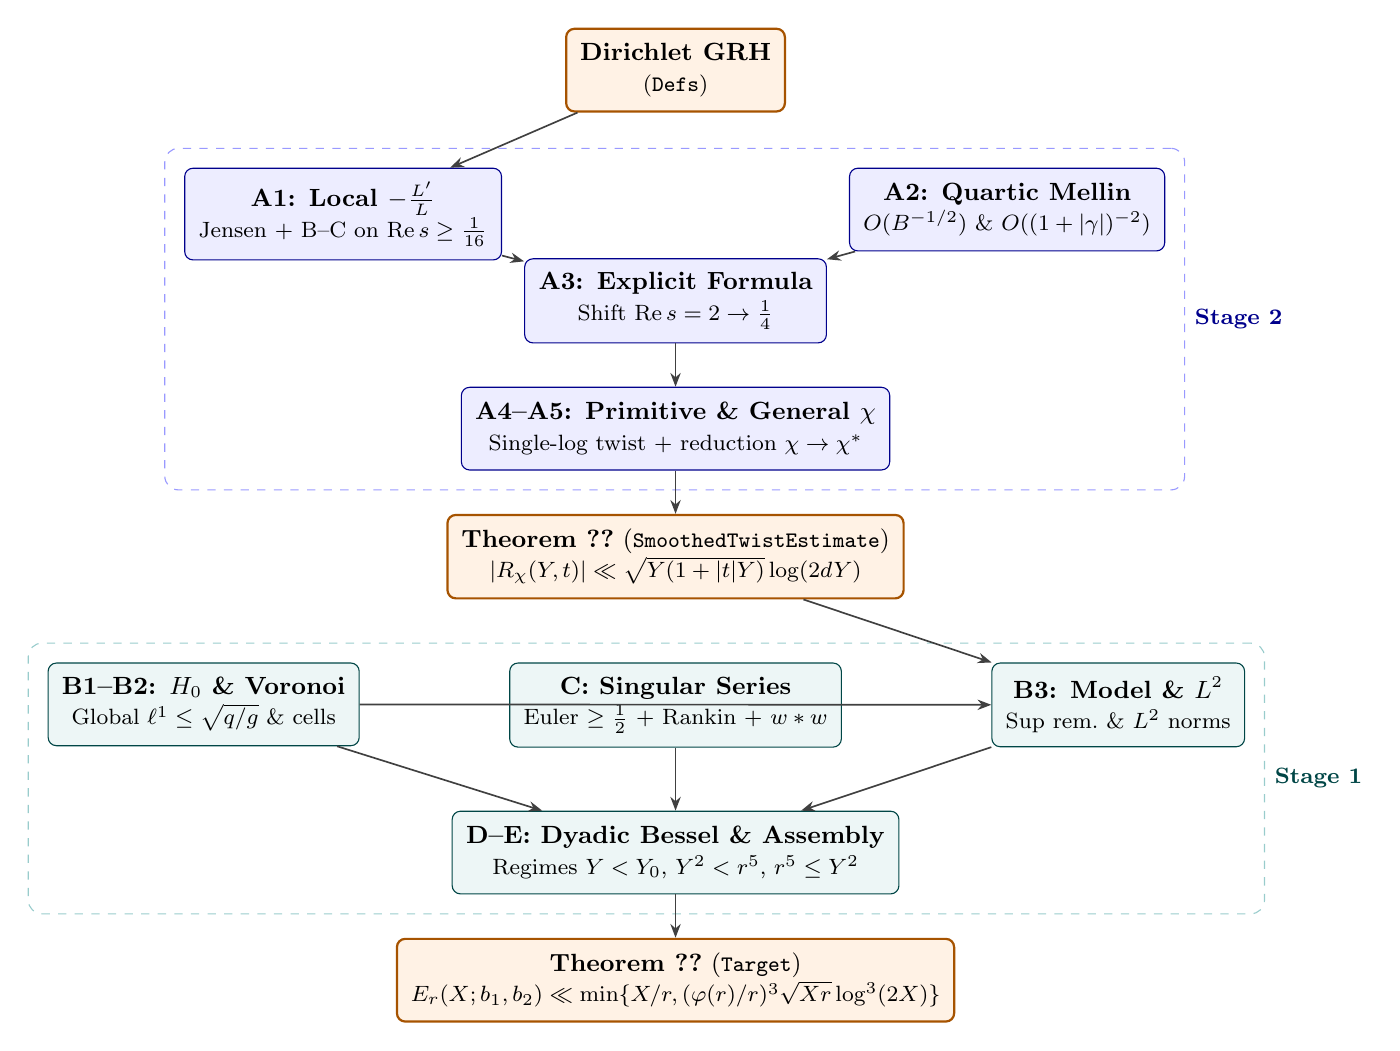
\begin{tikzpicture}[
  node distance=0.55cm and 0.65cm,
  box/.style={draw, rounded corners=3pt, align=center, font=\small, inner sep=5pt, minimum height=1.05cm},
  s2/.style={box, fill=blue!7, draw=blue!55!black},
  s1/.style={box, fill=teal!7, draw=teal!55!black},
  iface/.style={box, draw=orange!65!black, thick, fill=orange!10},
  arr/.style={-{Stealth[length=5pt]}, semithick, draw=black!75}
]
  % Stage 2
  \node[iface] (grh) {\textbf{Dirichlet \GRH{}}\\ \footnotesize(\lean{Defs})};
  \node[s2, below left=0.7cm and 0.8cm of grh] (a1) {\textbf{A1: Local $-\frac{L'}{L}$}\\ \footnotesize Jensen + B--C on $\Re s \ge \frac{1}{16}$};
  \node[s2, below right=0.7cm and 0.8cm of grh] (a2) {\textbf{A2: Quartic Mellin}\\ \footnotesize $O(B^{-1/2})$ \& $O((1+|\gamma|)^{-2})$};
  \node[s2, below=1.85cm of grh] (a3) {\textbf{A3: Explicit Formula}\\ \footnotesize Shift $\Re s = 2 \to \frac{1}{4}$};
  \node[s2, below=0.55cm of a3] (a4) {\textbf{A4--A5: Primitive \& General $\chi$}\\ \footnotesize Single-log twist + reduction $\chi \to \chi^*$};
  \node[iface, below=0.55cm of a4] (tw) {\textbf{Theorem~\ref{thm:smoothed-twist}} (\lean{SmoothedTwistEstimate})\\ \footnotesize $|R_\chi(Y,t)| \ll \sqrt{Y(1+|t|Y)}\log(2dY)$};

  % Stage 1
  \node[s1, below left=0.8cm and 1.1cm of tw] (b12) {\textbf{B1--B2: $H_0$ \& Voronoi}\\ \footnotesize Global $\ell^1 \le \sqrt{q/g}$ \& cells};
  \node[s1, below=0.8cm of tw] (c12) {\textbf{C: Singular Series}\\ \footnotesize Euler $\ge \frac{1}{2}$ + Rankin + $w*w$};
  \node[s1, below right=0.8cm and 1.1cm of tw] (b3) {\textbf{B3: Model \& $L^2$}\\ \footnotesize Sup rem.\ \& $L^2$ norms};
  \node[s1, below=0.8cm of c12] (d) {\textbf{D--E: Dyadic Bessel \& Assembly}\\ \footnotesize Regimes $Y<Y_0$, $Y^2<r^5$, $r^5 \le Y^2$};
  \node[iface, below=0.55cm of d] (tgt) {\textbf{Theorem~\ref{thm:main}} (\lean{Target})\\ \footnotesize $E_r(X;b_1,b_2) \ll \min\{X/r, (\varphi(r)/r)^3\sqrt{Xr}\log^3(2X)\}$};

  % Arrows
  \draw[arr] (grh) -- (a1);
  \draw[arr] (a1) -- (a3);
  \draw[arr] (a2) -- (a3);
  \draw[arr] (a3) -- (a4);
  \draw[arr] (a4) -- (tw);

  \draw[arr] (tw) -- (b3);
  \draw[arr] (b12) -- (b3);
  \draw[arr] (b12) -- (d);
  \draw[arr] (c12) -- (d);
  \draw[arr] (b3) -- (d);
  \draw[arr] (d) -- (tgt);

  \begin{scope}[on background layer]
    \node[draw=blue!40, dashed, rounded corners=5pt, fit=(a1)(a2)(a3)(a4), inner sep=7pt,
          label={[font=\footnotesize\bfseries, text=blue!55!black]right:Stage 2}] {};
    \node[draw=teal!40, dashed, rounded corners=5pt, fit=(b12)(c12)(b3)(d), inner sep=7pt,
          label={[font=\footnotesize\bfseries, text=teal!55!black]right:Stage 1}] {};
  \end{scope}
\end{tikzpicture}%
}
\caption{Two-stage modular proof architecture separating the conditional $L$-function analysis (Stage~2, Sections~\ref{sec:local-logderiv}--\ref{sec:explicit-formula}) from the composite Farey circle method (Stage~1, Sections~\ref{sec:char-voronoi}--\ref{sec:dyadic}) across the single-logarithm interface of Theorem~\ref{thm:smoothed-twist}.}
\label{fig:architecture}
\end{figure}

Figure~\ref{fig:architecture} summarizes the two-stage decomposition. Stage~2 (Sections~\ref{sec:local-logderiv}--\ref{sec:explicit-formula}) proves Theorem~\ref{thm:smoothed-twist} from Dirichlet \GRH{}, while Stage~1 (Sections~\ref{sec:char-voronoi}--\ref{sec:dyadic}) deduces Theorem~\ref{thm:main} unconditionally from Theorem~\ref{thm:smoothed-twist}.

% ==============================================================================
\section{Right-Half-Plane Local Zero Counts and Logarithmic Derivative Bounds}
\label{sec:local-logderiv}
% ==============================================================================

Throughout this section, let $d \ge 1$ and let $\chi \bmod d$ be a \emph{primitive} Dirichlet character. We work exclusively in the right half-plane $\Re s > 0$. Define the pole-cancelled completed $L$-function $F_\chi : \C \to \C$ by
\begin{equation}\label{eq:entireL}
  F_\chi(s) := \begin{cases}
    (s - 1)\zeta(s) & \text{if } \chi = 1 \text{ (so } d = 1\text{), with } F_1(1) := 1,\\
    L(s, \chi) & \text{if } \chi \neq 1,
  \end{cases}
\end{equation}
and set $\D_\chi(s) := -L'(s, \chi)/L(s, \chi)$. Because $\chi$ is primitive, $F_\chi$ is an entire function (\lean{entireL}), and by the classical non-vanishing of $L(s, \chi)$ on $\Re s \ge 1$ together with Dirichlet \GRH{}, every zero $\rho$ of $F_\chi$ in $\{\Re s > 0\}$ satisfies $\Re \rho = 1/2$. Denote the multiplicity of a zero $\rho$ of $F_\chi$ by $m_\rho := \ord_\rho(F_\chi) \in \N$ (\lean{zeroMult}).

\subsection{Elementary growth and center lower bound in \texorpdfstring{$\Re s \ge 1/16$}{Re s >= 1/16}}

Fix any $T \in \R$ and center $c := 2 + iT$, and consider the three concentric disks of radii
\begin{equation}\label{eq:radii}
  r_1 := \frac{7}{4} < r_2 := \frac{15}{8} < r_3 := \frac{31}{16} < 2.
\end{equation}
Notice that the largest closed disk $\overline{D}(c, r_3)$ lies completely inside the half-plane $\{\Re s \ge 1/16\}$; in particular, it avoids $\Re s \le 0$ altogether.

\begin{lemma}[Center lower bound and right-half-plane growth; \lean{norm\_entireL\_two\_add\_ge\_quarter}, \lean{norm\_entireL\_le}]
\label{lem:growth-and-center}
Let $\chi \bmod d$ be primitive and $T \in \R$.
\begin{enumerate}[label=(\alph*)]
  \item At the center $c = 2 + iT$, one has $|F_\chi(c)| \ge 1/4$.
  \item For every $s \in \C$ with $\Re s \ge 1/16$,
  \begin{equation}\label{eq:entireL-poly-bound}
    |F_\chi(s)| \le 16\, d\,(1 + |s|)^2.
  \end{equation}
  In particular, for every $z \in \overline{D}(2+iT, 31/16)$,
  \[
    |F_\chi(z)| \le 400\, d\,(2 + |T|)^2.
  \]
\end{enumerate}
\end{lemma}

\begin{proof}
For (a), the Dirichlet series $L(c, \chi) = \sum_{n \ge 1} \chi(n) n^{-c}$ converges absolutely at $\Re c = 2$, with first term $\chi(1) = 1$ and tail bounded by
\[
  \bigl|L(c, \chi) - 1\bigr| \le \sum_{n \ge 2} \frac{1}{n^2} = \frac{\pi^2}{6} - 1 \le \frac{3}{4},
\]
so $|L(c, \chi)| \ge 1/4$ without invoking Euler products. When $\chi = 1$, we also have $|c - 1| = |1 + iT| \ge 1$, giving $|F_1(c)| = |c-1|\cdot|\zeta(c)| \ge 1/4$.

For (b), write $A_\chi(x) := \sum_{1 \le n \le x} \chi(n)$. If $\chi \neq 1$, orthogonality over complete periods modulo~$d$ gives $|A_\chi(x)| \le d$ for all $x \ge 1$. On $\Re s > 1$, partial summation gives
\[
  L(s, \chi) = s \int_1^\infty A_\chi(x) x^{-s-1}\,dx.
\]
The integral on the right converges locally uniformly and defines a holomorphic function on all of $\{\Re s > 0\}$; by the identity theorem, the equality persists for $\Re s > 0$. For $\Re s \ge 1/16$, we deduce
\[
  |L(s, \chi)| \le |s| \cdot d \int_1^\infty x^{-\Re s - 1}\,dx = \frac{d |s|}{\Re s} \le 16\, d |s| \le 16\, d\,(1 + |s|)^2.
\]
When $\chi = 1$ ($d = 1$), substituting $\lfloor x \rfloor = x - \{x\}$ into $\zeta(s) = s \int_1^\infty \lfloor x\rfloor x^{-s-1}\,dx$ on $\Re s > 1$ yields
\[
  (s - 1)\zeta(s) = s - s(s - 1)\int_1^\infty \{x\}\, x^{-s-1}\,dx,
\]
which again extends analytically to $\{\Re s > 0\}$ and matches $F_1(1) = 1$. Since $0 \le \{x\} < 1$, on $\Re s \ge 1/16$ we obtain
\[
  |F_1(s)| \le |s| + \frac{|s|\cdot|s-1|}{\Re s} \le |s| + 16\,|s|\,(1+|s|) \le 16\,(1+|s|)^2.
\]
Finally, for $z \in \overline{D}(2+iT, 31/16)$ we have $|z| \le |2+iT| + 2 \le 4 + |T|$, hence $1 + |z| \le 5 + |T| \le \frac{5}{2}(2+|T|)$, and therefore $|F_\chi(z)| \le 16\cdot (5/2)^2\, d(2+|T|)^2 = 100\, d(2+|T|)^2 \le 400\, d(2+|T|)^2$.
\end{proof}

\subsection{Local zero count via Jensen's formula}

For any disk $D(c, r)$, let $Z_\chi(c, r)$ denote the finite set of zeros of $F_\chi$ in $\overline{D}(c, r)$, and let $N_\chi(c, r) := \sum_{\rho \in Z_\chi(c, r)} m_\rho$ be their count with multiplicity.

\begin{proposition}[Local zero count; \lean{diskZeroCount\_le}, \lean{zeroCount\_unit}]
\label{prop:zero-count}
Let $\chi \bmod d$ be primitive and $T \in \R$.
\begin{enumerate}[label=(\alph*)]
  \item Unconditionally, the zero count in $\overline{D}(2+iT, 15/8)$ satisfies
  \begin{equation}\label{eq:disk-zero-count}
    N_\chi\!\left(2+iT, \frac{15}{8}\right) \le 217 \log\bigl(2 d (2 + |T|)\bigr).
  \end{equation}
  \item Under Dirichlet \GRH{}, every zero $\rho$ of $F_\chi$ with $\Re \rho > 0$ and $|\Im \rho - T| \le 1$ lies in $\overline{D}(2+iT, 15/8)$. Consequently,
  \begin{equation}\label{eq:unit-zero-count}
    \sum_{\substack{\Re \rho > 0 \\ |\Im \rho - T| \le 1}} m_\rho \le 217 \log\bigl(2 d (2 + |T|)\bigr).
  \end{equation}
\end{enumerate}
\end{proposition}

\begin{proof}
By Jensen's formula applied to the entire function $F_\chi$ on the disk $\overline{D}(c, r_3)$ with $r_3 = 31/16$ and $F_\chi(c) \neq 0$,
\[
  \sum_{\rho \in Z_\chi(c, r_3)} m_\rho \log\!\left(\frac{r_3}{|\rho - c|}\right)
  = \frac{1}{2\pi}\int_0^{2\pi} \log\bigl|F_\chi(c + r_3 e^{i\theta})\bigr|\,d\theta - \log|F_\chi(c)|.
\]
Every term on the left is nonnegative, and restricting to $\rho \in Z_\chi(c, r_2)$ ($r_2 = 15/8$) yields $\log(r_3/|\rho - c|) \ge \log(r_3/r_2) = \log(31/30) > 1/31$. On the right, Lemma~\ref{lem:growth-and-center} gives
\[
  \frac{|F_\chi(c + r_3 e^{i\theta})|}{|F_\chi(c)|} \le 1600\, d\,(2 + |T|)^2 \le \bigl(2 d (2 + |T|)\bigr)^7
\]
since $2 d (2+|T|) \ge 4$ implies $(2 d(2+|T|))^5 \ge 4^5 = 1024$ and $4 \cdot 1024 \ge 1600$ (checking $1600 \cdot d(2+|T|)^2 \le (2d(2+|T|))^7$ directly: $1600 \le 2^7 \cdot 2^5 = 4096$). Dividing by $\log(31/30) > 1/31$ gives $N_\chi(c, 15/8) \le 31 \cdot 7 \log(2d(2+|T|)) = 217 \log(2d(2+|T|))$.

For (b), under Dirichlet \GRH{} any zero with $\Re \rho > 0$ has $\Re \rho = 1/2$, so if $|\Im \rho - T| \le 1$ then
\[
  |\rho - (2+iT)|^2 = \left(\frac{3}{2}\right)^2 + |\Im \rho - T|^2 \le \frac{9}{4} + 1 = \frac{13}{4} < \frac{225}{64} = \left(\frac{15}{8}\right)^2. \qedhere
\]
\end{proof}

\subsection{Local partial-fraction approximation and contour bounds}

To approximate $\D_\chi(s) = -L'(s, \chi)/L(s, \chi)$ on the inner disk $\overline{D}(c, 7/4)$, we extract the finite Blaschke-type polynomial factor carrying all zeros in $\overline{D}(c, 15/8)$ and apply Borel--Carath\'eodory to the logarithm of the non-vanishing remainder.

\begin{proposition}[Local partial-fraction formula; \lean{local\_negLogDeriv\_approx}]
\label{prop:local-approx}
Let $\chi \bmod d$ be primitive, $T \in \R$, and $c = 2 + iT$. Uniformly for all $s \in \overline{D}(c, 7/4)$ that are neither zeros of $F_\chi$ nor equal to $1$ (when $\chi = 1$),
\begin{equation}\label{eq:local-approx}
  \left|\D_\chi(s) - \frac{\1_{\chi=1}}{s-1} + \sum_{\rho \in Z_\chi(c, 15/8)} \frac{m_\rho}{s - \rho}\right|
  \le C_1 \log\bigl(2 d (2 + |T|)\bigr)
\end{equation}
with an explicit absolute constant $C_1$ (specifically $C_1 = 812{,}000$ in the formalization).
\end{proposition}

\begin{proof}
Define the polynomial $P(z) := \prod_{\rho \in Z_\chi(c, r_2)} (z - \rho)^{m_\rho}$. Since $F_\chi$ is entire, dividing out each zero of multiplicity $m_\rho$ yields an entire function $g : \C \to \C$ (\lean{extract\_zeros\_on\_closedBall}) such that $F_\chi(z) = P(z) g(z)$ everywhere and $g(z) \neq 0$ for all $z \in \overline{D}(c, r_2)$.

We bound $|g(z)/g(c)|$ on $\overline{D}(c, r_2)$ via the maximum modulus principle on the larger circle $|z - c| = r_3 = 31/16$. For every $\rho \in Z_\chi(c, r_2)$ and $|z - c| = r_3$, we have
\[
  |z - \rho| \ge r_3 - r_2 = \frac{1}{16}, \qquad |c - \rho| \le r_2 < 2,
\]
so $|(c - \rho)/(z - \rho)| \le 32$. Multiplying over all $\rho \in Z_\chi(c, r_2)$ gives $|P(c)/P(z)| \le 32^{N_\chi(c, r_2)}$. Therefore, on the circle $|z - c| = r_3$, Lemma~\ref{lem:growth-and-center} and Proposition~\ref{prop:zero-count}(a) imply
\[
  \left|\frac{g(z)}{g(c)}\right| = \left|\frac{F_\chi(z)}{F_\chi(c)}\right|\cdot\left|\frac{P(c)}{P(z)}\right|
  \le 1600\, d(2+|T|)^2 \cdot 32^{217 \log(2d(2+|T|))}
  \le \exp\bigl(A \log(2d(2+|T|))\bigr)
\]
for an explicit absolute constant $A > 0$. By the maximum modulus principle, the same upper bound holds throughout $\overline{D}(c, r_3)$ and in particular on $\overline{D}(c, r_2)$.

Because $g$ is holomorphic and non-vanishing on an open neighborhood $D(c, r_2')$ ($r_2' > r_2$) of the convex closed disk $\overline{D}(c, r_2)$, the holomorphic function $g'/g$ admits a holomorphic primitive $h$ on $D(c, r_2')$ normalized by $h(c) = 0$. Then $\frac{d}{dz}(g(z) e^{-h(z)}) = 0$, so $g(z)/g(c) = e^{h(z)}$ on $\overline{D}(c, r_2)$, whence
\[
  \Re h(z) = \log\left|\frac{g(z)}{g(c)}\right| \le A \log\bigl(2 d (2 + |T|)\bigr) \qquad \bigl(z \in \overline{D}(c, r_2)\bigr).
\]
Applying the Borel--Carath\'eodory theorem on $D(c, r_2)$ with intermediate radius $r_2^* := \frac{1}{2}(r_1 + r_2) = 29/16$ gives
\[
  \sup_{|z - c| \le r_2^*} |h(z)| \le \frac{2 r_2^*}{r_2 - r_2^*} A \log\bigl(2 d (2 + |T|)\bigr) = 58 A \log\bigl(2 d (2 + |T|)\bigr).
\]
Now Cauchy's integral estimate for $h' = g'/g$ on the disk $D(s, r_2^* - r_1) = D(s, 1/16) \subset D(c, r_2^*)$ for any $s \in \overline{D}(c, r_1)$ yields
\[
  \left|\frac{g'(s)}{g(s)}\right| = |h'(s)| \le 16 \cdot 58 A \log\bigl(2 d (2 + |T|)\bigr).
\]
Finally, differentiating $F_\chi = P g$ gives
\[
  -\frac{F_\chi'(s)}{F_\chi(s)} = -\sum_{\rho \in Z_\chi(c, r_2)} \frac{m_\rho}{s - \rho} - \frac{g'(s)}{g(s)},
\]
and since $-\frac{F_\chi'(s)}{F_\chi(s)} = \D_\chi(s) - \frac{\1_{\chi=1}}{s-1}$, the bound~\eqref{eq:local-approx} follows.
\end{proof}

Proposition~\ref{prop:local-approx} immediately yields both contour estimates required for Stage~2: the single-logarithm bound on the vertical line $\Re s = 1/4$, and the $\log^2$ bound on symmetric horizontal segments at well-chosen heights.

\begin{corollary}[Single-logarithm bound on $\Re s = 1/4$; \lean{negLogDeriv\_quarter}]
\label{cor:quarter-line}
Assume Dirichlet \GRH{}. For every primitive $\chi \bmod d$ and every $u \in \R$,
\begin{equation}\label{eq:quarter-line}
  \left|\D_\chi\!\left(\tfrac{1}{4} + i u\right)\right| \le C_2 \log\bigl(2 d (2 + |u|)\bigr),
\end{equation}
where $C_2$ is an absolute constant ($C_2 = 812{,}870$ in the formalization).
\end{corollary}

\begin{proof}
Apply Proposition~\ref{prop:local-approx} with $T = u$ and $s = 1/4 + iu$. Since $|s - c| = 7/4 = r_1$, \eqref{eq:local-approx} applies. Under \GRH{}, every zero $\rho \in Z_\chi(c, 15/8)$ lies in $\{\Re z > 0\}$ and therefore satisfies $\Re \rho = 1/2$, whence $|s - \rho| \ge |\Re s - \Re \rho| = 1/4$. Moreover $|s - 1| \ge 3/4$. Summing the zero contributions via Proposition~\ref{prop:zero-count}(a) yields
\[
  \left|\D_\chi\!\left(\tfrac{1}{4} + iu\right)\right|
  \le \frac{4}{3} + 4 N_\chi\!\left(2+iu, \tfrac{15}{8}\right) + C_1 \log\bigl(2d(2+|u|)\bigr)
  \le (C_1 + 870) \log\bigl(2d(2+|u|)\bigr). \qedhere
\]
\end{proof}

\begin{proposition}[Good horizontal heights; \lean{exists\_good\_height}]
\label{prop:good-height}
Assume Dirichlet \GRH{}. For every primitive $\chi \bmod d$ and every integer $j \ge 2$, there exists a real height $T \in [j, j+1]$ such that $F_\chi(s) \neq 0$ whenever $\Re s > 0$ and $\Im s \in \{T, -T\}$, and uniformly for all $\sigma \in [1/4, 2]$,
\begin{equation}\label{eq:good-height}
  \max\Bigl\{\bigl|\D_\chi(\sigma + iT)\bigr|,\; \bigl|\D_\chi(\sigma - iT)\bigr|\Bigr\}
  \le C_3 \log^2\bigl(2 d (2 + T)\bigr),
\end{equation}
with an absolute constant $C_3$ ($C_3 = 4 \times 10^6$ in the formalization).
\end{proposition}

\begin{proof}
Complex characters $\chi$ need not have zeros symmetric about the real axis, so collect both the ordinates $\Im\rho$ from $Z_\chi(2+ij,15/8)$ and the reflected ordinates $-\Im\rho$ from $Z_\chi(2-ij,15/8)$ that lie in $[j,j+1]$. Proposition~\ref{prop:zero-count}(b) ensures that these include all the absolute ordinates of critical-strip zeros in $[j,j+1]$. By Proposition~\ref{prop:zero-count}(a), their number $M$ satisfies
\[
  M \le 434 \log\bigl(2 d (2 + j)\bigr).
\]
Choose $T$ as the midpoint of a longest gap between the collected points and the endpoints $j,j+1$. The gap has length at least $1/(M+1)$. Separation from the endpoints also covers ordinates outside the interval, so
\[
  \min\bigl\{|T - \Im \rho|,\; |-T - \Im \rho|\bigr\} \ge \frac{1}{2(M+1)} \ge \frac{1}{900 \log(2d(2+j))}
\]
for every zero $\rho$ with $\Re\rho>0$. Applying Proposition~\ref{prop:local-approx} at $c_\pm=2\pm iT$ (where $|\sigma\pm iT-c_\pm|\le7/4$ and $|\sigma\pm iT-1|\ge T\ge2$) gives
\[
  \bigl|\D_\chi(\sigma \pm iT)\bigr|
  \le \frac{1}{2} + 900 \log\bigl(2d(2+j)\bigr) \cdot 217 \log\bigl(2d(2+T)\bigr) + C_1 \log\bigl(2d(2+T)\bigr),
\]
which yields~\eqref{eq:good-height} since $\log(2d(2+T)) \ge \log 8 > 1$.
\end{proof}

% ==============================================================================
\section{Uniform Oscillatory Estimates for the Quartic Mellin Kernel}
\label{sec:quartic-mellin}
% ==============================================================================

The results of this section are completely unconditional and independent of \GRH{}. For any real frequency $\lambda \in \R$, put $B := 1 + |\lambda|$ and define the tilted quartic Mellin kernel
\begin{equation}\label{eq:K-def}
  K_\lambda(s) := \int_0^1 w(x)\, \e(\lambda x)\, x^{s-1}\,dx = 16 \int_0^1 x^{s+1}(1-x)^2\, \e(\lambda x)\,dx.
\end{equation}
For $Y \ge 1$ and $t \in \R$, let $f_{Y,t}(x) := w(x/Y)\e(t x)$ (\lean{scaledTiltedBump}). A scaling $x \mapsto Y x$ relates the Mellin transform $\widetilde{f}_{Y,t}(s) := \int_0^\infty f_{Y,t}(x) x^{s-1}\,dx$ directly to $K_\lambda$ with $\lambda = t Y$:
\begin{equation}\label{eq:mellin-scaling}
  \widetilde{f}_{Y,t}(s) = Y^s K_{tY}(s) \qquad (\Re s > -2).
\end{equation}
Because $|w(x)\e(\lambda x)x^{s-1}| \le 16 x^{\Re s + 1}$ on $(0, 1)$, the integral~\eqref{eq:K-def} converges absolutely and defines a holomorphic function on $\{\Re s > -2\}$ (\lean{differentiableOn\_quarticKernel}). At $\lambda = 0$, elementary integration gives the exact normalization check
\begin{equation}\label{eq:K0-exact}
  K_0(s) = \frac{32}{(s+2)(s+3)(s+4)} \quad (\Re s > -2), \qquad K_0(1) = \frac{8}{15}
\end{equation}
(\lean{quarticKernel\_zero}, \lean{quarticKernel\_zero\_one}), and at $s = 1$ we have $\widetilde{f}_{Y,t}(1) = Y K_{tY}(1) = \int_0^Y f_{Y,t}(x)\,dx$.

\subsection{Logarithmic coordinates and second-derivative oscillatory bound}

Writing $s = \sigma + i\gamma$ with $1/4 \le \sigma \le 2$ and substituting $x = e^u$ ($u \in (-\infty, 0]$), we rewrite~\eqref{eq:K-def} as
\begin{equation}\label{eq:K-log-coords}
  K_\lambda(\sigma + i\gamma) = \int_{-\infty}^0 a_\sigma(u)\, e^{i\phi(u)}\,du,
\end{equation}
where the amplitude and complete phase are
\begin{equation}\label{eq:amp-phase}
  a_\sigma(u) := 16\, e^{(\sigma+2)u}(1 - e^u)^2, \qquad \phi(u) := \gamma u + 2\pi \lambda e^u.
\end{equation}
Note that $a_\sigma(0) = a_\sigma'(0) = 0$ and all derivatives of $a_\sigma$ decay like $O(e^{(\sigma+2)u})$ as $u \to -\infty$, while
\begin{equation}\label{eq:phase-derivs}
  \phi'(u) = \gamma + 2\pi\lambda e^u, \qquad \phi''(u) = \phi'''(u) = 2\pi\lambda e^u.
\end{equation}

We isolate a completely elementary second-derivative Van der Corput lemma tailored for formalization.

\begin{lemma}[Second-derivative oscillatory integral bound; \lean{van\_der\_corput\_second\_deriv}]
\label{lem:vdc}
Let $p \le q$, $m > 0$, $A \ge 0$, $V \ge 0$, and let $a, \phi \in C^2([p, q], \R)$ satisfy:
\begin{enumerate}[label=(\roman*)]
  \item $|a(u)| \le A$ for all $u \in [p, q]$ and $\int_p^q |a'(u)|\,du \le V$;
  \item either $\phi''(u) \ge m$ for all $u \in [p, q]$, or $\phi''(u) \le -m$ for all $u \in [p, q]$.
\end{enumerate}
Then
\begin{equation}\label{eq:vdc}
  \left|\int_p^q a(u)\, e^{i\phi(u)}\,du\right| \le \frac{8 A + V}{\sqrt{m}}.
\end{equation}
\end{lemma}

\begin{proof}
By complex conjugation we may assume $\phi''(u) \ge m$ throughout $[p, q]$. Set $\delta := \sqrt{m}$. Because $\phi'$ is strictly increasing with $\phi'(u) - \phi'(v) \ge m(u - v)$ for $u \ge v$, the set $I_0 := \{u \in [p, q] : |\phi'(u)| \le \delta\}$ is a (possibly empty) closed subinterval $[c_1, c_2] \subset [p, q]$ of length $c_2 - c_1 \le 2\delta/m = 2/\sqrt{m}$. On $I_0$, the trivial bound gives $\left|\int_{c_1}^{c_2} a(u)e^{i\phi(u)}\,du\right| \le 2 A / \sqrt{m}$.

On the left wing $[p, c_1]$ (when $p < c_1$), we have $\phi'(u) \le -\delta < 0$. Integrating by parts via $e^{i\phi(u)} = \frac{1}{i\phi'(u)}\frac{d}{du}(e^{i\phi(u)})$ gives
\[
  \int_p^{c_1} a(u) e^{i\phi(u)}\,du
  = \left[\frac{a(u)}{i\phi'(u)}e^{i\phi(u)}\right]_p^{c_1}
    - \int_p^{c_1} \left(\frac{a'(u)}{i\phi'(u)} - \frac{a(u)\phi''(u)}{i\phi'(u)^2}\right) e^{i\phi(u)}\,du.
\]
Using $|\phi'(u)| \ge \delta = \sqrt{m}$ and the monotonicity identity $\int_p^{c_1} \frac{\phi''(u)}{\phi'(u)^2}\,du = \frac{1}{\phi'(p)} - \frac{1}{\phi'(c_1)} \le \frac{1}{\delta}$, the triangle inequality yields
\[
  \left|\int_p^{c_1} a(u) e^{i\phi(u)}\,du\right|
  \le \frac{2A}{\sqrt{m}} + \frac{1}{\sqrt{m}}\int_p^{c_1} |a'(u)|\,du + \frac{A}{\sqrt{m}}
  = \frac{3A + \int_p^{c_1}|a'(u)|\,du}{\sqrt{m}}.
\]
The same bound holds on the right wing $[c_2, q]$ where $\phi'(u) \ge \delta$. Summing the three pieces and using $\int_p^{c_1}|a'| + \int_{c_2}^q |a'| \le V$ gives~\eqref{eq:vdc}.
\end{proof}

\begin{proposition}[Uniform frequency decay; \lean{quarticKernel\_norm\_le\_inv\_sqrt}]
\label{prop:K-uniform}
Uniformly for all $\lambda \in \R$, $\gamma \in \R$, and $\sigma \in [1/4, 2]$,
\begin{equation}\label{eq:K-uniform}
  \bigl|K_\lambda(\sigma + i\gamma)\bigr| \le \frac{1792}{\sqrt{1 + |\lambda|}}.
\end{equation}
\end{proposition}

\begin{proof}
For $|\lambda| \le 1$, the trivial bound $|K_\lambda(\sigma+i\gamma)| \le \int_0^1 16 x^{\sigma+1}\,dx \le 16$ already implies~\eqref{eq:K-uniform} since $16\sqrt{2} < 1792$.

Assume now $|\lambda| > 1$. Decompose $(-\infty, 0] = \bigcup_{j=0}^\infty I_j$ into dyadic blocks $I_j := [-(j+1)\log 2, -j\log 2]$, on which $2^{-(j+1)} \le e^u \le 2^{-j}$. On $I_j$:
\begin{itemize}
  \item $|a_\sigma(u)| \le 16 e^{(\sigma+2)u} \le 16 \cdot 2^{-j(\sigma+2)} \le 16 \cdot 2^{-9j/4}$;
  \item $|a_\sigma'(u)| \le 16(\sigma + 4)e^{(\sigma+2)u} \le 96 \cdot 2^{-9j/4}$, so $\int_{I_j} |a_\sigma'(u)|\,du \le 96 (\log 2)\, 2^{-9j/4}$;
  \item $|\phi''(u)| = 2\pi|\lambda| e^u \ge \pi |\lambda|\, 2^{-j}$ with constant sign throughout $I_j$.
\end{itemize}
Applying Lemma~\ref{lem:vdc} on each $I_j$ yields
\[
  \left|\int_{I_j} a_\sigma(u) e^{i\phi(u)}\,du\right|
  \ll \frac{2^{-9j/4}}{\sqrt{\pi |\lambda| 2^{-j}}}
  = \frac{2^{-7j/4}}{\sqrt{\pi |\lambda|}}.
\]
Summing the geometric series over $j \ge 0$ (which converges with ratio $2^{-7/4} < 1/3$) and noting $|\lambda| \ge \frac{1}{2}(1 + |\lambda|)$ for $|\lambda| > 1$ completes the proof.
\end{proof}

\subsection{Uniform tail decay via full-phase double integration by parts}

The second pillar of preserving the single logarithm in Theorem~\ref{thm:smoothed-twist} is an $O((1+|\gamma|)^{-2})$ tail bound whose implied constant is \emph{completely independent of $\lambda$}.

\begin{proposition}[Uniform vertical tail bound; \lean{quarticKernel\_norm\_le\_tail}]
\label{prop:K-tail}
Uniformly for all $\lambda \in \R$, $\sigma \in [1/4, 2]$, and all $\gamma \in \R$ satisfying $|\gamma| \ge 4\pi|\lambda| + 2$,
\begin{equation}\label{eq:K-tail}
  \bigl|K_\lambda(\sigma + i\gamma)\bigr| \le \frac{60{,}000}{(1 + |\gamma|)^2}.
\end{equation}
\end{proposition}

\begin{proof}
Fix $\sigma \in [1/4, 2]$ and $|\gamma| \ge 4\pi|\lambda| + 2$. For all $u \le 0$, since $0 < e^u \le 1$, we have $2\pi|\lambda| e^u \le |\gamma|/2$, and hence
\begin{equation}\label{eq:phase-lower}
  |\phi'(u)| = |\gamma + 2\pi\lambda e^u| \ge |\gamma| - 2\pi|\lambda| \ge \frac{|\gamma|}{2}.
\end{equation}
Crucially, because we leave $2\pi\lambda e^u$ inside the phase $\phi(u)$, the derivatives of $1/\phi'(u)$ satisfy bounds \emph{uniform in $\lambda$}:
\[
  \left|\frac{1}{\phi'(u)}\right| \le \frac{2}{|\gamma|}, \qquad
  \left|\left(\frac{1}{\phi'}\right)'(u)\right| = \frac{|\phi''(u)|}{|\phi'(u)|^2} \le \frac{|\gamma|/2}{(|\gamma|/2)^2} = \frac{2}{|\gamma|},
\]
and
\[
  \left|\left(\frac{1}{\phi'}\right)''(u)\right|
  = \left|\frac{-\phi'''(u)}{\phi'(u)^2} + \frac{2\phi''(u)^2}{\phi'(u)^3}\right|
  \le \frac{|\gamma|/2}{(|\gamma|/2)^2} + \frac{2(|\gamma|/2)^2}{(|\gamma|/2)^3}
  = \frac{6}{|\gamma|}.
\]
Define the differential operator $L(f) := \frac{d}{du}\bigl(f / (i\phi')\bigr)$. On any truncated interval $[-M, 0]$ ($M > 0$), two integrations by parts using $e^{i\phi(u)} = \frac{1}{i\phi'(u)}\frac{d}{du}(e^{i\phi(u)})$ yield
\begin{align*}
  \int_{-M}^0 a_\sigma(u) e^{i\phi(u)}\,du
  &= \left[\frac{a_\sigma(u)}{i\phi'(u)}e^{i\phi(u)} - \frac{L(a_\sigma)(u)}{i\phi'(u)}e^{i\phi(u)}\right]_{-M}^0
     + \int_{-M}^0 L^2(a_\sigma)(u)\, e^{i\phi(u)}\,du.
\end{align*}
At the upper endpoint $u = 0$, we have $a_\sigma(0) = 0$ and $a_\sigma'(0) = 0$, hence $L(a_\sigma)(0) = 0$ as well: \emph{both} boundary terms at $u = 0$ vanish identically. As $M \to \infty$, both $a_\sigma(-M)$ and $a_\sigma'(-M)$ decay like $O(e^{-(\sigma+2)M}) \to 0$, so the lower boundary terms also vanish in the limit.

Expanding $L^2(a_\sigma)$ by the product rule shows that
\[
  \bigl|L^2(a_\sigma)(u)\bigr|
  \le \frac{C_0}{|\gamma|^2}\Bigl(|a_\sigma''(u)| + |a_\sigma'(u)| + |a_\sigma(u)|\Bigr)
\]
for an explicit absolute constant $C_0$ independent of $\lambda$ and $\sigma \in [1/4, 2]$. Since $|a_\sigma(u)|$, $|a_\sigma'(u)|$, and $|a_\sigma''(u)|$ are all $O(e^{9u/4})$ uniformly for $\sigma \in [1/4, 2]$ and $\int_{-\infty}^0 e^{9u/4}\,du = 4/9$, integrating over $(-\infty, 0]$ yields $|K_\lambda(\sigma + i\gamma)| \ll |\gamma|^{-2} \ll (1+|\gamma|)^{-2}$ (using $|\gamma| \ge 2 \implies 1 + |\gamma| \le \frac{3}{2}|\gamma|$, which gives the explicit constant $60{,}000$ verified in Lean).
\end{proof}

\begin{corollary}[Mellin inversion on $\Re s = 2$; \lean{mellinInv\_scaledTiltedBump\_eq}]
\label{cor:mellin-inv}
For every $Y \ge 1$, $t \in \R$, and $\sigma \in [1/4, 2]$, the function $u \mapsto \widetilde{f}_{Y,t}(\sigma + iu)$ belongs to $L^1(\R)$. Moreover, for every $x > 0$,
\begin{equation}\label{eq:mellin-inv}
  f_{Y,t}(x) = \frac{1}{2\pi} \int_{-\infty}^\infty \widetilde{f}_{Y,t}(2 + iu)\, x^{-(2+iu)}\,du.
\end{equation}
\end{corollary}

\begin{proof}
Vertical integrability follows directly from Proposition~\ref{prop:K-tail} together with continuity of $K_{tY}(\sigma+iu)$. The function $f_{Y,t}$ is continuous, is supported in $[0,Y]$, and vanishes quadratically at $0$. The weighted function $x \mapsto x^{\sigma-1} f_{Y,t}(x)$ is therefore integrable on $(0,\infty)$ for the stated $\sigma$. Mathlib's Mellin inversion theorem (\lean{mellinInv\_mellin\_eq}) gives~\eqref{eq:mellin-inv}.
\end{proof}

% ==============================================================================
\section{Smoothed Explicit Formula and Proof of Theorem~\ref{thm:smoothed-twist}}
\label{sec:explicit-formula}
% ==============================================================================

We now combine Sections~\ref{sec:local-logderiv} and~\ref{sec:quartic-mellin} by shifting a single vertical contour from $\Re s = 2$ to $\Re s = 1/4$, first for primitive characters and then for arbitrary characters $\chi \bmod d$.

\begin{figure}[htbp]
\centering
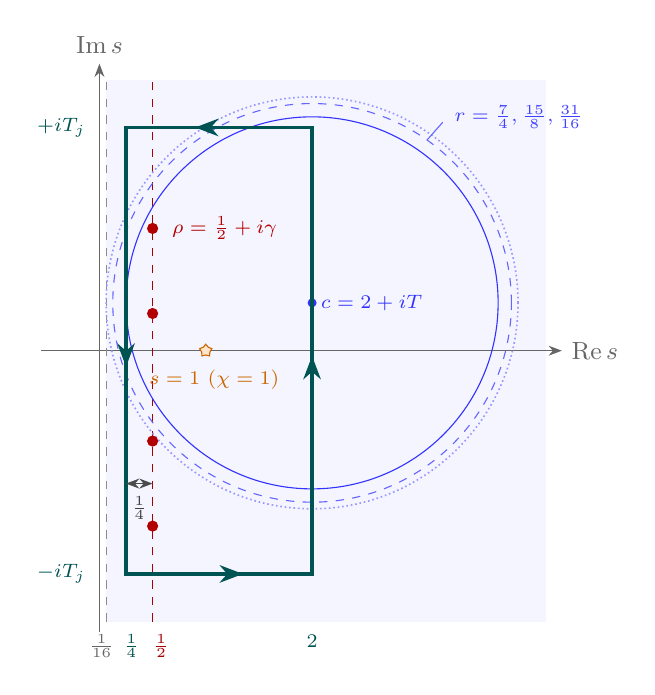
\begin{tikzpicture}[scale=1.35]
  % True-to-scale isotropic coordinates: (sigma, gamma)
  % Shaded safe half-plane Re s >= 1/16
  \fill[blue!4] (0.0625,-2.55) rectangle (4.2,2.55);
  % Axes
  \draw[-{Stealth}, thin, black!60] (-0.55,0) -- (4.35,0) node[right, font=\small] {$\Re s$};
  \draw[-{Stealth}, thin, black!60] (0,-2.65) -- (0,2.7) node[above, font=\small] {$\Im s$};

  % Vertical reference lines
  \draw[dashed, black!45] (0.0625,-2.55) -- (0.0625,2.55);
  \node[below, font=\scriptsize, black!60] at (0.02,-2.58) {$\frac{1}{16}$};

  \draw[dashed, red!65!black, semithick] (0.5,-2.55) -- (0.5,2.55);
  \node[below, font=\scriptsize, red!65!black] at (0.58,-2.58) {$\frac{1}{2}$};

  % Three true-to-scale concentric disks around c = 2 + 0.45i:
  % r1 = 7/4 = 1.75 (tangent to Re s = 1/4), r2 = 15/8 = 1.875, r3 = 31/16 = 1.9375 (tangent to Re s = 1/16)
  \coordinate (C) at (2.0, 0.45);
  \draw[blue!40, densely dotted, semithick] (C) circle (1.9375);
  \draw[blue!60, dashed] (C) circle (1.875);
  \draw[blue!80] (C) circle (1.75);
  \fill[blue!80] (C) circle (1.2pt) node[right=2pt, font=\scriptsize, fill=blue!4, inner sep=1pt] {$c = 2+iT$};
  \node[font=\scriptsize, blue!75, anchor=west] at (3.25, 2.2) {$r = \frac{7}{4}, \frac{15}{8}, \frac{31}{16}$};
  \draw[thin, blue!60] (3.23, 2.15) -- (3.08, 1.98);

  % Contour rectangle: [1/4, 2] x [-2.1, 2.1]
  \draw[very thick, teal!65!black] (0.25,-2.1) -- (2.0,-2.1) -- (2.0,2.1) -- (0.25,2.1) -- cycle;
  % Orientation arrows
  \draw[-{Stealth}, very thick, teal!65!black] (2.0,-0.6) -- (2.0,-0.05);
  \draw[-{Stealth}, very thick, teal!65!black] (1.35,2.1) -- (0.9,2.1);
  \draw[-{Stealth}, very thick, teal!65!black] (0.25,0.4) -- (0.25,-0.15);
  \draw[-{Stealth}, very thick, teal!65!black] (0.9,-2.1) -- (1.35,-2.1);

  \node[below, font=\scriptsize, teal!65!black] at (0.30,-2.58) {$\frac{1}{4}$};
  \node[below, font=\scriptsize, teal!65!black] at (2.0,-2.58) {$2$};
  \node[left, font=\scriptsize, teal!65!black] at (-0.04,2.1) {$+iT_j$};
  \node[left, font=\scriptsize, teal!65!black] at (-0.04,-2.1) {$-iT_j$};

  % Zeros on Re s = 1/2
  \foreach \y in {-1.65, -0.85, 0.35, 1.15} {
    \fill[red!70!black] (0.5, \y) circle (1.5pt);
  }
  \node[right=2pt, font=\scriptsize, red!70!black] at (0.54, 1.15) {$\rho = \frac{1}{2}+i\gamma$};

  % Pole at s = 1 (principal character)
  \node[draw=orange!80!black, fill=orange!20, star, star points=5, inner sep=1.1pt] (pole) at (1.0, 0) {};
  \node[below, font=\scriptsize, orange!80!black] at (1.08, -0.09) {$s=1$ ($\chi=1$)};

  % Distance annotation between Re s = 1/4 and Re s = 1/2
  \draw[{Stealth}-{Stealth}, thin, black!70] (0.25, -1.25) -- (0.5, -1.25);
  \node[below, font=\scriptsize, black!75] at (0.375, -1.28) {$\frac{1}{4}$};
\end{tikzpicture}
\caption{True-to-scale geometry of the right-half-plane contour shift from $\Re s = 2$ to $\Re s = 1/4$ at symmetric good heights $\pm i T_j$ (Section~\ref{sec:explicit-formula}). The three concentric disks centered at $c = 2+iT$ of radii $7/4 < 15/8 < 31/16$ lie completely inside the shaded half-plane $\{\Re s \ge 1/16\}$ (with the inner and outer circles tangent to $\Re s = 1/4$ and $\Re s = 1/16$, respectively); keeping the left edge at distance $1/4$ from the \GRH{} critical line $\Re s = 1/2$ preserves the single-logarithm bound.}
\label{fig:contour}
\end{figure}

\subsection{Elementary rectangular residue calculus and smoothed explicit formula}

For a rectangle $[x_1, x_2] \times [y_1, y_2]$ ($x_1 < x_2$, $y_1 < y_2$), define its positively oriented boundary integral by
\[
  \mathcal{I}_{x_1, x_2}^{y_1, y_2}(G)
  := \int_{x_1}^{x_2} G(x + i y_1)\,dx + i\int_{y_1}^{y_2} G(x_2 + i y)\,dy
     - \int_{x_1}^{x_2} G(x + i y_2)\,dx - i\int_{y_1}^{y_2} G(x_1 + i y)\,dy.
\]
We avoid invoking general homology or winding-number theorems by using a direct elementary residue identity for finitely many simple poles.

\begin{lemma}[Simple-pole rectangular residue formula; \lean{rectIntegral\_inv\_sub}, \lean{rectIntegral\_eq\_sum\_simple\_poles}]
\label{lem:rect-residue}
Let $x_1 < x_2$ and $y_1 < y_2$.
\begin{enumerate}[label=(\alph*)]
  \item For every interior point $p \in (x_1, x_2) \times (y_1, y_2)$, $\mathcal{I}_{x_1, x_2}^{y_1, y_2}\!\bigl(z \mapsto (z - p)^{-1}\bigr) = 2\pi i$.
  \item Let $S \subset (x_1, x_2) \times (y_1, y_2)$ be a finite set, let $c : S \to \C$, and suppose $G$ admits a decomposition $G(z) = H(z) + \sum_{p \in S} \frac{c(p)}{z - p}$ on $[x_1, x_2] \times [y_1, y_2] \setminus S$, where $H$ is continuous on the closed rectangle and holomorphic on the open rectangle. Then
  \[
    \mathcal{I}_{x_1, x_2}^{y_1, y_2}(G) = 2\pi i \sum_{p \in S} c(p).
  \]
\end{enumerate}
\end{lemma}

\begin{proof}
For (a), writing $p = a + ib$ with $x_1 < a < x_2$ and $y_1 < b < y_2$, antiderivatives with respect to the edge parameters are $\frac{1}{2}\log((x-a)^2 + (y-b)^2) - i\arctan\!\bigl(\frac{x-a}{y-b}\bigr)$ on horizontal edges and $\frac{1}{2}\log((x-a)^2 + (y-b)^2) + i\arctan\!\bigl(\frac{y-b}{x-a}\bigr)$ on vertical edges. All logarithmic terms cancel pairwise at the four corners, and applying the complementary identity $\arctan(u) + \arctan(1/u) = \pm\pi/2$ at each corner sums the imaginary parts to $4 \cdot (\pi/2) = 2\pi$.

For (b), linearity of $\mathcal{I}_{x_1, x_2}^{y_1, y_2}$ reduces to $\mathcal{I}_{x_1, x_2}^{y_1, y_2}(H) = 0$, which holds by Cauchy--Goursat's theorem on rectangles (already in Mathlib as \lean{Complex.integral\_boundary\_rect\_eq\_zero\_of\_differentiable\_on\_off\_countable}).
\end{proof}

\begin{theorem}[Smoothed explicit formula for primitive characters; \lean{primitive\_smoothed\_explicit\_formula}]
\label{thm:explicit-formula}
Assume Dirichlet \GRH{}. Let $\chi \bmod d$ be primitive, $Y \ge 2$, and $t \in \R$. Then the series $\sum_{\rho : \Re \rho > 0} m_\rho \widetilde{f}_{Y,t}(\rho)$ converges absolutely, the function $u \mapsto \widetilde{f}_{Y,t}(1/4+iu)\D_\chi(1/4+iu)$ belongs to $L^1(\R)$, and
\begin{align}\label{eq:explicit-formula}
  \sum_{1 \le n \le Y} \Lambda(n)\chi(n) w\!\left(\frac{n}{Y}\right) \e(tn)
  &= \1_{\chi=1} \widetilde{f}_{Y,t}(1)
    - \sum_{\Re \rho > 0} m_\rho \widetilde{f}_{Y,t}(\rho) \nonumber\\
  &\quad + \frac{1}{2\pi} \int_{-\infty}^\infty \widetilde{f}_{Y,t}\!\left(\tfrac{1}{4}+iu\right) \D_\chi\!\left(\tfrac{1}{4}+iu\right) du.
\end{align}
\end{theorem}

\begin{proof}
We first express the left-hand side as a vertical integral on $\Re s = 2$ (\lean{smoothedPrimeSum\_eq\_verticalIntegral}). Since $f_{Y,t}(n) = 0$ for $n > Y$, applying Corollary~\ref{cor:mellin-inv} to each $n \ge 1$ and summing against $\Lambda(n)\chi(n)$ gives
\[
  \sum_{1 \le n \le Y} \Lambda(n)\chi(n) f_{Y,t}(n)
  = \frac{1}{2\pi} \sum_{n=1}^\infty \int_{-\infty}^\infty \Lambda(n)\chi(n) n^{-(2+iu)} \widetilde{f}_{Y,t}(2+iu)\,du.
\]
Since $\sum_{n=1}^\infty \Lambda(n) n^{-2} < \infty$ and $\widetilde{f}_{Y,t}(2+i\cdot) \in L^1(\R)$, Fubini's theorem justifies interchanging sum and integral. Identifying $\sum_{n=1}^\infty \Lambda(n)\chi(n) n^{-s} = \D_\chi(s)$ on $\Re s > 1$ (\lean{LSeries\_twist\_vonMangoldt\_eq}) gives
\begin{equation}\label{eq:line-2}
  \sum_{1 \le n \le Y} \Lambda(n)\chi(n) f_{Y,t}(n)
  = \frac{1}{2\pi} \int_{-\infty}^\infty \widetilde{f}_{Y,t}(2+iu)\, \D_\chi(2+iu)\,du.
\end{equation}

Next, partition the critical-strip zeros into unit vertical bands $B_k := \{\rho : \Re \rho > 0,\; k \le \Im \rho < k+1\}$ ($k \in \Z$). By Dirichlet \GRH{}, every $\rho \in B_k$ satisfies $\Re \rho = 1/2$, so $|\widetilde{f}_{Y,t}(\rho)| = Y^{1/2}|K_{tY}(1/2+i\Im \rho)|$. Combining Proposition~\ref{prop:zero-count}(b) with Proposition~\ref{prop:K-uniform} (for small $|k|$) and Proposition~\ref{prop:K-tail} (for $|k| \ge 4\pi|t|Y + 3$) yields
\[
  \sum_{\rho \in B_k} m_\rho \bigl|\widetilde{f}_{Y,t}(\rho)\bigr|
  \ll \frac{Y^{1/2} \log(2d(2+|k|))}{(1+|k|)^2} \qquad (|k| \ge 4\pi|t|Y + 3),
\]
which is summable over $k \in \Z$ (\lean{summable\_norm\_zeroTerm}). Similarly, Corollary~\ref{cor:quarter-line} and Proposition~\ref{prop:K-tail} show $|\widetilde{f}_{Y,t}(1/4+iu)\D_\chi(1/4+iu)| \ll Y^{1/4}(1+|u|)^{-2}\log(2d(2+|u|))$ for large $|u|$, establishing $L^1(\R)$ integrability on $\Re s = 1/4$ (\lean{integrable\_quarter\_line}).

Now apply Proposition~\ref{prop:good-height} for each integer $j \ge 2$ to pick a height $T_j \in [j, j+1]$ free of zeros on $\Im s = \pm T_j$. Set $G(s) := \widetilde{f}_{Y,t}(s)\D_\chi(s)$. Inside the rectangle $[1/4, 2] \times [-T_j, T_j]$, the singularities of $G$ are precisely the finite set $S_j$ of zeros $\rho$ of $F_\chi$ with $|\Im \rho| < T_j$ (all lying on $\Re s = 1/2$ by \GRH{}, each producing a simple pole of $\D_\chi$ with residue $-m_\rho$, hence residue $-m_\rho \widetilde{f}_{Y,t}(\rho)$ for $G$) together with a simple pole at $s = 1$ with residue $\widetilde{f}_{Y,t}(1)$ when $\chi = 1$. Factoring $F_\chi$ on a disk containing the rectangle (as in Proposition~\ref{prop:local-approx}) shows that $H_j(s) := G(s) - \frac{\1_{\chi=1}\widetilde{f}_{Y,t}(1)}{s-1} + \sum_{\rho \in S_j} \frac{m_\rho \widetilde{f}_{Y,t}(\rho)}{s-\rho}$ extends holomorphically across every point of the closed rectangle. Lemma~\ref{lem:rect-residue}(b) therefore gives
\begin{equation}\label{eq:rect-j}
  \frac{1}{2\pi i}\,\mathcal{I}_{1/4, 2}^{-T_j, T_j}(G) = \1_{\chi=1}\widetilde{f}_{Y,t}(1) - \sum_{\rho \in S_j} m_\rho \widetilde{f}_{Y,t}(\rho).
\end{equation}
On the two horizontal segments $s = \sigma \pm i T_j$ ($1/4 \le \sigma \le 2$), once $T_j \ge 4\pi|t|Y + 2$, Propositions~\ref{prop:good-height} and~\ref{prop:K-tail} give
\[
  \left|\int_{1/4}^2 G(\sigma \pm i T_j)\,d\sigma\right|
  \ll Y^2 \cdot \frac{\log^2(2d(2+T_j))}{(1+T_j)^2} \longrightarrow 0 \qquad (j \to \infty).
\]
Meanwhile, the two vertical edges converge to the improper integrals over $\R$ by dominated convergence, and the finite sum $\sum_{\rho \in S_j} m_\rho \widetilde{f}_{Y,t}(\rho)$ converges to $\sum_{\Re\rho > 0} m_\rho \widetilde{f}_{Y,t}(\rho)$ by absolute summability. Letting $j \to \infty$ in~\eqref{eq:rect-j} and substituting~\eqref{eq:line-2} yields~\eqref{eq:explicit-formula}.
\end{proof}

\subsection{Bounding the explicit-formula terms and reduction from imprimitive characters}

\begin{proposition}[Primitive smoothed twist estimate; \lean{primitive\_smoothedTwist\_bound}]
\label{prop:primitive-twist}
Assume Dirichlet \GRH{}. There is an absolute constant $C_{\mathrm{prim}} > 0$ ($C_{\mathrm{prim}} = 6 \times 10^{11}$ in Lean) such that for every primitive $\chi \bmod d$, every $Y \ge 2$, and every $t \in [-1/2, 1/2]$,
\[
  \bigl|R_\chi(Y, t)\bigr| \le C_{\mathrm{prim}} \sqrt{Y\bigl(1 + |t| Y\bigr)}\,\log(2 d Y).
\]
\end{proposition}

\begin{proof}
Set $B := 1 + |t|Y$, $L := \log(2dY) \ge \log 4 > 1$, and $R_0 := 4\pi|t|Y + 3 \le 16 B$. Since $|t| \le 1/2$ and $Y \ge 2$, we have $1 \le B \le 1 + Y/2 \le Y$. By Theorem~\ref{thm:explicit-formula},
\begin{align}
  R_\chi(Y, t)
  &= \1_{\chi=1}\!\left(\int_0^Y f_{Y,t}(x)\,dx - \sum_{n=1}^Y f_{Y,t}(n)\right)
     - \sum_{\Re \rho > 0} m_\rho \widetilde{f}_{Y,t}(\rho) \nonumber\\
  &\quad + \frac{1}{2\pi}\int_{-\infty}^\infty \widetilde{f}_{Y,t}\!\left(\tfrac{1}{4}+iu\right) \D_\chi\!\left(\tfrac{1}{4}+iu\right) du.
  \label{eq:rem-decomp}
\end{align}
We bound the three terms in~\eqref{eq:rem-decomp} separately.

\emph{1. Principal-character discretization error (no Euler--Maclaurin needed).}
Since $f_{Y,t}(Y) = 0$ and $f_{Y,t}(x) = w(x/Y)\e(tx)$, splitting $[0, Y] = \bigcup_{n=1}^Y [n-1, n]$ gives
\[
  \left|\int_0^Y f_{Y,t}(x)\,dx - \sum_{n=1}^Y f_{Y,t}(n)\right|
  \le \sum_{n=1}^Y \int_{n-1}^n \bigl|f_{Y,t}(x) - f_{Y,t}(n)\bigr|\,dx.
\]
For $x \in [n-1, n]$, the triangle inequality, the Lipschitz bound $|w(u) - w(v)| \le 4|u - v|$ (\lean{quarticBump\_lipschitz}), and $|\e(tx) - \e(tn)| \le 2\pi|t||x-n| \le 2\pi|t|$ yield
\[
  \bigl|f_{Y,t}(x) - f_{Y,t}(n)\bigr| \le \frac{4}{Y} + 2\pi|t| \le \frac{8 B}{Y}.
\]
Summing over $1 \le n \le Y$ gives $\le 8 B$ (\lean{principal\_integral\_sub\_sum\_le}). Since $B \le Y$, we have $B \le \sqrt{YB} \le \sqrt{YB}\,L$, so this error is absorbed with huge room to spare.

\emph{2. Sum over critical-strip zeros.}
Grouping zeros into unit bands $B_k$ ($k \in \Z$) and applying Propositions~\ref{prop:zero-count}(b), \ref{prop:K-uniform}, and~\ref{prop:K-tail}, we split into inner bands $|k| \le R_0$ and outer bands $|k| > R_0$:
\begin{itemize}
  \item For $|k| \le R_0 \le 16 B \le 16 Y$, we have $2 + |k| \le 18 Y$, so $\log(2d(2+|k|)) \le 4 \log(2dY) = 4L$. There are at most $2\lfloor R_0 \rfloor + 1 \le 33 B$ inner bands, each contributing $\ll \sqrt{Y} B^{-1/2} \cdot L$, for a total of $\ll \sqrt{Y B}\, L$.
  \item For $|k| > R_0$, we use the elementary inequality $\log(2d(2+|k|)) \le 5 L \sqrt{1 + |k|}$ (\lean{log\_two\_d\_add\_le\_five\_log\_sqrt}), so each outer band contributes $\ll \sqrt{Y} L (1 + |k|)^{-3/2}$. Since $\sum_{k \in \Z} (1+|k|)^{-3/2} \le 6$ (proved via the telescoping bound $(1+n)^{-3/2} \le 2/\sqrt{n} - 2/\sqrt{n+1}$), the entire outer tail contributes $\ll \sqrt{Y} L \le \sqrt{Y B}\, L$.
\end{itemize}
Combining both parts gives $\bigl|\sum_{\rho} m_\rho \widetilde{f}_{Y,t}(\rho)\bigr| \ll \sqrt{YB}\, L$ (\lean{norm\_tsum\_zeroTerm\_le}).

\emph{3. Vertical line integral on $\Re s = 1/4$.}
Splitting $\R$ at $|u| \le R_0$ and $|u| > R_0$ and using Corollary~\ref{cor:quarter-line} in place of the unit-band zero count (together with $\int_{\R} (1+|u|)^{-3/2}\,du = 4$) gives identically
\[
  \left|\frac{1}{2\pi}\int_{-\infty}^\infty \widetilde{f}_{Y,t}\!\left(\tfrac{1}{4}+iu\right) \D_\chi\!\left(\tfrac{1}{4}+iu\right) du\right|
  \ll Y^{1/4}\sqrt{B}\, L \le \sqrt{Y B}\, L
\]
(\lean{norm\_quarter\_integral\_le}). Summing the three bounds proves Proposition~\ref{prop:primitive-twist}.
\end{proof}

\begin{proof}[Proof of Theorem~\ref{thm:smoothed-twist}]
Let $\chi \bmod d$ be any Dirichlet character, and let $\chi^* \bmod d^*$ be its associated primitive character, with conductor $d^* \mid d$. First, $\chi = 1$ if and only if $d^* = 1$, which holds if and only if $\chi^* = 1$ (\lean{eq\_one\_iff\_primitiveCharacter\_eq\_one}). Hence the indicator $\1_{\chi=1}$ cancels identically in the difference $R_\chi(Y, t) - R_{\chi^*}(Y, t)$. Moreover, whenever $\gcd(n, d) = 1$ we have $\chi(n) = \chi^*(n)$, so
\[
  R_\chi(Y, t) - R_{\chi^*}(Y, t)
  = \sum_{\substack{1 \le n \le Y \\ \gcd(n, d) > 1}} \Lambda(n)\bigl(\chi(n) - \chi^*(n)\bigr)\, w\!\left(\frac{n}{Y}\right) \e(tn).
\]
Since $|\chi(n) - \chi^*(n)| \le 2$, $0 \le w \le 1$, and $|\e(tn)| = 1$, we obtain
\begin{equation}\label{eq:imprim-diff}
  \bigl|R_\chi(Y, t) - R_{\chi^*}(Y, t)\bigr|
  \le 2 \sum_{\substack{1 \le n \le Y \\ \gcd(n, d) > 1}} \Lambda(n)
  = 2 \sum_{p \mid d} \sum_{p^k \le Y} \log p
  \le 2 \sum_{p \mid d} \frac{\log Y}{\log p}\,\log p
  = 2\,\omega(d)\log Y.
\end{equation}
Because $2^{\omega(d)} \le d$ implies $\omega(d) \le \frac{\log d}{\log 2} \le 2\log(2d)$ (\lean{nonCoprimeVonMangoldt\_le}), and $\log Y = 2\log\sqrt{Y} \le 2\sqrt{Y} \le 2\sqrt{Y(1+|t|Y)}$, the discrepancy~\eqref{eq:imprim-diff} is bounded by
\[
  4\log(2d)\log Y \le 8 \sqrt{Y(1 + |t|Y)}\,\log(2 d Y)
\]
(\lean{norm\_smoothedTiltedRemainder\_sub\_primitive\_le}). Combining this with Proposition~\ref{prop:primitive-twist} applied to $\chi^* \bmod d^*$ and noting $\log(2d^* Y) \le \log(2dY)$ yields Theorem~\ref{thm:smoothed-twist} with $C_{\mathrm{tw}} = C_{\mathrm{prim}} + 8$.
\end{proof}

% ==============================================================================
\section{Global \texorpdfstring{$H_0$}{H0}-Invariance Character Expansion and Weighted Farey--Voronoi Cells}
\label{sec:char-voronoi}
% ==============================================================================

We now begin Stage~1 of the proof: deducing Theorem~\ref{thm:main} unconditionally from Theorem~\ref{thm:smoothed-twist}. The two structural ingredients needed to handle arbitrary composite moduli $r \ge 1$ without prime-factorization case splits are the global $H_0$-subgroup character expansion and the weighted Farey--Voronoi partition of the circle.

\subsection{Global \texorpdfstring{$H_0$}{H0}-invariance character \texorpdfstring{$\ell^1$}{l1} bound}

Fix arbitrary positive integers $r, q \ge 1$, and put $g := \gcd(r, q)$ and $L_0 := \lcm(r, q) = rq/g$. Let $a, b \in \Z$ satisfy $\gcd(a, q) = \gcd(b, r) = 1$. On the finite abelian group $G := (\Z/rq\Z)^\times$, consider the supported additive character
\[
  f(u) := \1_{u \equiv b \pmod r}\, \e\!\left(\frac{a u}{r q}\right), \qquad u \in G.
\]
By Fourier inversion on $G$, we expand $f(u) = \sum_{\chi \bmod rq} c_\chi \chi(u)$ with character coefficients
\begin{equation}\label{eq:char-coeff}
  c_\chi := \frac{1}{\varphi(rq)} \sum_{\substack{u \in (\Z/rq\Z)^\times \\ u \equiv b \pmod r}} \e\!\left(\frac{a u}{r q}\right)\overline{\chi(u)}.
\end{equation}

\begin{lemma}[Global $H_0$-invariance character bound; \lean{charCoeff\_one\_eq\_zero\_of\_one\_lt\_gcd}, \lean{charCoeff\_one\_coprime}, \lean{charCoeff\_l1\_le\_sharp}]
\label{lem:char-l1}
For all positive integers $r, q \ge 1$ and integers $a, b$ with $\gcd(a, q) = \gcd(b, r) = 1$:
\begin{enumerate}[label=(\alph*)]
  \item If $g = \gcd(r, q) > 1$, then $c_{\chi_0} = 0$ (the principal-character coefficient vanishes).
  \item If $\gcd(r, q) = 1$, then letting $\bar{r}$ denote a multiplicative inverse of $r$ modulo~$q$,
  \[
    \e\!\left(-\frac{a b}{r q}\right) c_{\chi_0}
    = \e\!\left(-\frac{a \bar{r} b}{q}\right)\frac{\mu(q)}{\varphi(r)\varphi(q)}.
  \]
  \item For all $r, q \ge 1$ simultaneously,
  \begin{equation}\label{eq:char-l1-sharp}
    \sum_{\chi \bmod rq} |c_\chi|
    \le \sqrt{\frac{\varphi(rq)}{g\,\varphi(r)}}
    \le \sqrt{\frac{q}{\gcd(r, q)}}.
  \end{equation}
\end{enumerate}
\end{lemma}

\begin{proof}
Define the subset $H_0 := \{1 + m L_0 \bmod rq : m \in \Z/g\Z\} \subset \Z/rq\Z$. Because every prime dividing $rq$ divides $L_0 = \lcm(r, q)$, each $1 + m L_0$ is coprime to $rq$, so $H_0 \subset G$. Moreover,
\[
  L_0^2 = (rq)\cdot \frac{r}{g}\cdot \frac{q}{g} \equiv 0 \pmod{rq},
\]
so $(1 + m_1 L_0)(1 + m_2 L_0) \equiv 1 + (m_1 + m_2) L_0 \pmod{rq}$. Hence $H_0 \cong \Z/g\Z$ is a subgroup of $G$ of exact order~$g$ (generated by \lean{hGen r q}).

Now take any $u \in \supp(f)$ (so $r \mid (u - b)$) and any $h = 1 + m L_0 \in H_0$. Since $r \mid L_0$, we have $uh \equiv u \equiv b \pmod r$, so $uh \in \supp(f)$. Since $q \mid L_0$ and $r \mid (u-b)$, we have $rq \mid (u-b)L_0$, whence
\[
  u h = u + m b L_0 + m(u - b)L_0 \equiv u + m b L_0 \pmod{rq}.
\]
Because $L_0 / (rq) = 1/g$, this yields the exact equivariance law
\[
  f(u h) = \e\!\left(\frac{a u + a m b L_0}{rq}\right) = \e\!\left(\frac{a b}{g}\, m\right) f(u) =: \psi_0(h)\, f(u),
\]
where $\psi_0 : H_0 \to \C^\times$ is a character of $H_0$. Because $\gcd(a, q) = 1$ and $\gcd(b, r) = 1$, we have $\gcd(ab, g) = 1$, so $\psi_0$ is a primitive character of $H_0$; in particular, $\psi_0 \neq 1$ whenever $g > 1$.

Substituting $u \mapsto u h$ in~\eqref{eq:char-coeff} gives $c_\chi = \psi_0(h)\overline{\chi(h)}\, c_\chi$ for all $h \in H_0$. Consequently,
\begin{equation}\label{eq:char-fiber}
  c_\chi \neq 0 \implies \chi|_{H_0} = \psi_0.
\end{equation}
If $g > 1$, the principal character $\chi_0$ satisfies $\chi_0|_{H_0} = 1 \neq \psi_0$, proving~(a).

For~(b), when $\gcd(r, q) = 1$, the Chinese remainder theorem identifies $\{u \in G : u \equiv b \bmod r\}$ with $v \in (\Z/q\Z)^\times$ via $u \equiv b + r(v - b)\bar{r} \pmod{rq}$ (where $r\bar{r} \equiv 1 \pmod q$). Then $a(u - b)/(rq) \equiv a\bar{r}(v - b)/q \pmod 1$, so
\[
  \e\!\left(-\frac{ab}{rq}\right) c_{\chi_0}
  = \frac{1}{\varphi(r)\varphi(q)}\,\e\!\left(-\frac{a\bar{r}b}{q}\right)\sum_{v \in (\Z/q\Z)^\times} \e\!\left(\frac{a\bar{r}v}{q}\right)
  = \e\!\left(-\frac{a\bar{r}b}{q}\right)\frac{\mu(q)}{\varphi(r)\varphi(q)},
\]
since $\gcd(a\bar{r}, q) = 1$ implies $c_q(a\bar{r}) = \mu(q)$.

For~(c), the restriction map $\widehat{G} \to \widehat{H_0}$ is a surjective group homomorphism (equivalently, every non-empty fiber over $\psi_0$ has cardinality $|G|/|H_0| = \varphi(rq)/g$; in Lean this is proved directly without Pontryagin duality by fixing one element of the fiber and translating by the kernel $\{\chi : \chi|_{H_0} = 1\}$, which bijects with $\widehat{G/H_0}$). By~\eqref{eq:char-fiber}, at most $\varphi(rq)/g$ coefficients $c_\chi$ are nonzero. Meanwhile, the reduction map $(\Z/rq\Z)^\times \twoheadrightarrow (\Z/r\Z)^\times$ is surjective, so $|\supp(f)| = \varphi(rq)/\varphi(r)$. By Parseval's identity on~$G$,
\[
  \sum_{\chi \bmod rq} |c_\chi|^2 = \frac{1}{\varphi(rq)}\sum_{u \in G} |f(u)|^2 = \frac{|\supp(f)|}{\varphi(rq)} = \frac{1}{\varphi(r)}.
\]
Applying Cauchy--Schwarz over the $\le \varphi(rq)/g$ nonzero terms gives
\[
  \sum_{\chi \bmod rq} |c_\chi|
  \le \sqrt{\frac{\varphi(rq)}{g} \cdot \frac{1}{\varphi(r)}}
  = \sqrt{\frac{\varphi(rq)}{g\,\varphi(r)}}.
\]
Finally, since $\varphi(rq) \le q\varphi(r)$ (every prime dividing $rq$ either divides $r$, contributing a factor $p$ to $\varphi(rq)/\varphi(r)$, or does not divide $r$, contributing $p - 1 < p$), we obtain $\sqrt{\varphi(rq)/(g\varphi(r))} \le \sqrt{q/g}$.
\end{proof}

\subsection{Weighted Farey--Voronoi partition of the circle}

Rather than constructing explicit Farey mediants, we partition $\R$ (periodically modulo~$1$) into measurable weighted Voronoi cells around reduced fractions of denominator at most~$Q$. For any integer $Q \ge 1$, let
\[
  \mathcal{F}_Q := \bigl\{(q, a) \in \N \times \N : 1 \le q \le Q,\; 0 \le a < q,\; \gcd(a, q) = 1\bigr\}
\]
be the finite set of Farey centers, ordered lexicographically by $(q, a)$. For $c = (q, a) \in \mathcal{F}_Q$ and $\alpha \in \R$, define the weighted circular distance $d_c(\alpha) := q \|\alpha - a/q\|_\T$ and the Voronoi cell
\begin{equation}\label{eq:voronoi-cell}
  \V_Q(c) := \Bigl\{\alpha \in \R : \forall c' \in \mathcal{F}_Q,\; d_c(\alpha) < d_{c'}(\alpha) \text{ or } \bigl(d_c(\alpha) = d_{c'}(\alpha) \text{ and } c \le_{\mathrm{lex}} c'\bigr)\Bigr\}.
\end{equation}

\begin{lemma}[Weighted Farey--Voronoi radius sandwich; \lean{voronoiCell\_outer\_radius}, \lean{voronoiCell\_inner\_radius}]
\label{lem:voronoi}
For every integer $Q \ge 1$, the sets $\{\V_Q(c)\}_{c \in \mathcal{F}_Q}$ are $1$-periodic, measurable, pairwise disjoint, and partition $\R$. Moreover, for every $c = (q, a) \in \mathcal{F}_Q$:
\begin{enumerate}[label=(\alph*)]
  \item \emph{(Outer radius)} If $\alpha \in \V_Q(c)$, then $\|\alpha - a/q\|_\T \le \frac{1}{q Q}$.
  \item \emph{(Inner radius)} If $\|\alpha - a/q\|_\T < \frac{1}{2 q Q}$, then $\alpha \in \V_Q(c)$.
\end{enumerate}
\end{lemma}

\begin{proof}
Periodicity, measurability, disjointness, and covering follow immediately from the finiteness and total lexicographic order of $\mathcal{F}_Q$ together with the continuity of $\alpha \mapsto d_c(\alpha)$.

For~(a), Dirichlet's approximation theorem gives some $c_0 = (q_0, a_0) \in \mathcal{F}_Q$ with $q_0 \|\alpha - a_0/q_0\|_\T \le 1/Q$. Since $\alpha \in \V_Q(c)$, we have $q \|\alpha - a/q\|_\T = d_c(\alpha) \le d_{c_0}(\alpha) \le 1/Q$, so $\|\alpha - a/q\|_\T \le 1/(qQ)$.

For~(b), suppose $\|\alpha - a/q\|_\T < 1/(2qQ)$, so $d_c(\alpha) < 1/(2Q)$. For any distinct center $c' = (q', a') \in \mathcal{F}_Q$, the reduced fractions satisfy $\|a/q - a'/q'\|_\T \ge 1/(q q')$. By the triangle inequality on $\T$,
\[
  \left\|\alpha - \frac{a'}{q'}\right\|_\T \ge \frac{1}{q q'} - \frac{1}{2 q Q},
\]
and multiplying by $q' \le Q$ yields
\[
  d_{c'}(\alpha) \ge \frac{1}{q}\!\left(1 - \frac{q'}{2 Q}\right) \ge \frac{1}{2 q} \ge \frac{1}{2 Q} > d_c(\alpha),
\]
proving $\alpha \in \V_Q(c)$.
\end{proof}

% ==============================================================================
\section{Composite Circle-Method Analysis: Remainder, \texorpdfstring{$L^2$}{L2} Norms, and Singular Series}
\label{sec:circle-method}
% ==============================================================================

Fix a modulus $r \ge 1$, coprime residue classes $0 \le b_1, b_2 < r$, and a dyadic scale $Y \ge r$. Define the Farey cutoff and constant-ratio major-arc truncation level by
\begin{equation}\label{eq:Q-Q0}
  Q := \lfloor \sqrt{Y/r} \rfloor, \qquad Q_0 := \lfloor Q / 2^{24} \rfloor.
\end{equation}
For each center $c = (q, a) \in \mathcal{F}_Q$, define the model coefficient
\begin{equation}\label{eq:model-coeff}
  \kappa_{r,b}(c) := \begin{cases}
    \e\!\left(-\dfrac{a\bar{r} b}{q}\right)\dfrac{r}{\varphi(r)}\dfrac{\mu(q)}{\varphi(q)} & \text{if } \gcd(q, r) = 1,\\[8pt]
    0 & \text{if } \gcd(q, r) > 1,
  \end{cases}
\end{equation}
where $\bar{r}$ is the inverse of $r$ modulo~$q$, and define the truncated major-arc model on $\R$ by
\begin{equation}\label{eq:model-sum}
  M_b^{(w)}(\alpha) := \sum_{\substack{c = (q, a) \in \mathcal{F}_Q \\ q \le Q_0}} \1_{\V_Q(c)}(\alpha)\, \kappa_{r, b}(c)\, V_b^{(w)}\!\bigl(\operatorname{wrap}(\alpha - a/q)\bigr),
\end{equation}
where $V_b^{(w)}(\beta)$ is the smooth frequency kernel~\eqref{eq:V-def}. Note that because the Voronoi cells $\V_Q(c)$ are pairwise disjoint, at most one term in~\eqref{eq:model-sum} is nonzero at any $\alpha \in \R$.

\subsection{Elementary multiplicative bounds for \texorpdfstring{$m/\varphi(m)$}{m/phi(m)}}

In several places we use the following elementary power bound on $m/\varphi(m)$, which avoids Mertens' theorem and $\log\log$ bookkeeping completely while giving strict power savings.

\begin{lemma}[Elementary totient ratio bound; \lean{div\_totient\_le\_rpow\_sixteenth}, \lean{div\_totient\_le\_rpow\_eighth}]
\label{lem:totient-pow}
For every integer $m \ge 1$,
\[
  \frac{m}{\varphi(m)} \le 2^{16}\, m^{1/16} \qquad\text{and}\qquad \frac{m}{\varphi(m)} \le 2^{16}\, m^{1/8}.
\]
\end{lemma}

\begin{proof}
Write $m/\varphi(m) = \prod_{p \mid m} \frac{p}{p-1}$. For every prime $p \ge 17$, we have $(p/(p-1))^{16} \le (17/16)^{16} < e < 17 \le p$, and hence $p/(p-1) \le p^{1/16}$. The six primes $p \in \{2, 3, 5, 7, 11, 13\}$ satisfy $\prod_{p \le 13} \frac{p}{p-1} < 2^{16}$. Multiplying over all prime divisors $p \mid m$ yields
\[
  \frac{m}{\varphi(m)} \le 2^{16} \prod_{\substack{p \mid m \\ p \ge 17}} p^{1/16} \le 2^{16}\, m^{1/16} \le 2^{16}\, m^{1/8}. \qedhere
\]
\end{proof}

\subsection{Uniform \texorpdfstring{$L^\infty$}{L-infinity} bound on the remainder \texorpdfstring{$S_b^{(w)} - M_b^{(w)}$}{Sb - Mb}}

\begin{proposition}[Uniform remainder bound; \lean{remainder\_sup\_le}]
\label{prop:rem-sup}
Assume Theorem~\ref{thm:smoothed-twist} holds with constant $C_{\mathrm{tw}} > 0$. Suppose $1 \le r \le Y$, $0 \le b < r$ with $\gcd(b, r) = 1$, and $Q = \lfloor \sqrt{Y/r} \rfloor \ge 2^{25}$. Then uniformly for all $\alpha \in \R$,
\begin{equation}\label{eq:rem-sup}
  \bigl|S_b^{(w)}(\alpha) - M_b^{(w)}(\alpha)\bigr|
  \le C_{\mathrm{rem}}\, Y^{3/4} r^{-1/4} \log(2Y),
\end{equation}
where $C_{\mathrm{rem}} > 0$ depends only on $C_{\mathrm{tw}}$ (specifically $C_{\mathrm{rem}} = 6 C_{\mathrm{tw}} + 2^{288}$ in Lean).
\end{proposition}

\begin{proof}
Set $M := Y^{3/4} r^{-1/4}$. By Lemma~\ref{lem:voronoi}, any $\alpha \in \R$ belongs to a unique Voronoi cell $\V_Q(c)$ for some $c = (q, a) \in \mathcal{F}_Q$. Write $\beta := \operatorname{wrap}(\alpha - a/q)$, so that $|\beta| \le 1/(qQ) \le 1/2$ by Lemma~\ref{lem:voronoi}(a). Substituting $n = r j + b$ into~\eqref{eq:S-def} and factoring out the constant phase $\theta := \e(-ab/(rq) - \beta b/r)$ (with $|\theta| = 1$) gives
\[
  S_b^{(w)}(\alpha) = \theta \sum_{\substack{1 \le n \le Y \\ n \equiv b \pmod r}} w\!\left(\frac{n}{Y}\right) \varpi(n)\, \e\!\left(\frac{a n}{r q}\right)\e\!\left(\frac{\beta}{r}\, n\right).
\]
We compare this sum with $M_b^{(w)}(\alpha)$ in four elementary steps:

\emph{Step 1 (Prime powers).} Replacing $\varpi(n)$ by $\Lambda(n)$ incurs an error bounded by $\sum_{1 \le n \le Y} (\Lambda(n) - \varpi(n)) \le \sqrt{Y}\log Y \le M\log(2Y)$ (\lean{primePowerMass\_le}), since $r \le Y$ implies $\sqrt{Y} \le Y^{3/4}r^{-1/4} = M$.

\emph{Step 2 (Coprimality with $rq$).} Restricting the sum to $\gcd(n, rq) = 1$ drops only prime powers $p^k \le Y$ with $p \mid rq$. By~\eqref{eq:imprim-diff} (\lean{nonCoprimeVonMangoldt\_le}), this error is at most
\[
  2\log(2rq)\log Y \le 4\log^2(2Y) \ll M\log(2Y)
\]
(since $Y/r \ge Q^2 \ge 2^{50}$ forces $M = \sqrt{Y}(Y/r)^{1/4} \ge 2^{12.5}\sqrt{Y} \gg \log(2Y)$).

\emph{Step 3 (Character expansion and Theorem~\ref{thm:smoothed-twist}).} On $\{n \le Y : n \equiv b \bmod r,\; \gcd(n, rq) = 1\}$, Lemma~\ref{lem:char-l1} expands $\1_{n \equiv b \bmod r}\e(an/(rq)) = \sum_{\chi \bmod rq} c_\chi \chi(n)$, yielding
\begin{align*}
  &\sum_{\substack{1 \le n \le Y \\ n \equiv b \pmod r,\, \gcd(n, rq)=1}} w\!\left(\frac{n}{Y}\right)\Lambda(n)\e\!\left(\frac{an}{rq}\right)\e\!\left(\frac{\beta n}{r}\right) \\
  &\qquad = \sum_{\chi \bmod rq} c_\chi R_\chi\!\left(Y, \frac{\beta}{r}\right) + c_{\chi_0} \sum_{n=1}^Y w\!\left(\frac{n}{Y}\right)\e\!\left(\frac{\beta n}{r}\right).
\end{align*}
For the twist sum, since $|\beta/r| \le 1/(rqQ) \le 1/2$, Theorem~\ref{thm:smoothed-twist} and Lemma~\ref{lem:char-l1}(c) give
\begin{align*}
  \left|\sum_{\chi \bmod rq} c_\chi R_\chi\!\left(Y, \frac{\beta}{r}\right)\right|
  &\le \left(\sum_{\chi \bmod rq} |c_\chi|\right) \cdot C_{\mathrm{tw}} \sqrt{Y\!\left(1 + \frac{|\beta| Y}{r}\right)}\,\log(2 r q Y) \\
  &\le \sqrt{\frac{q}{\gcd(r,q)}} \cdot C_{\mathrm{tw}} \sqrt{Y\!\left(1 + \frac{Y}{r q Q}\right)} \cdot 3\log(2Y).
\end{align*}
Using $q \le Q \le \sqrt{Y/r}$ and $Q \ge \frac{1}{2}\sqrt{Y/r}$, we have
\[
  q Y\!\left(1 + \frac{Y}{r q Q}\right) = q Y + \frac{Y^2}{r Q} \le Y\sqrt{\frac{Y}{r}} + 2 Y\sqrt{\frac{Y}{r}} = 3 Y^{3/2} r^{-1/2} = 3 M^2,
\]
so the entire twist sum is bounded by $6 C_{\mathrm{tw}} M \log(2Y)$.

\emph{Step 4 (Principal term and constant-ratio cutoff $Q_0 = \lfloor Q/2^{24}\rfloor$).}
If $\gcd(q, r) > 1$, then $c_{\chi_0} = 0$ by Lemma~\ref{lem:char-l1}(a) and $M_b^{(w)}(\alpha) = 0$ by~\eqref{eq:model-coeff}, so the principal-term difference vanishes identically.

Assume now $\gcd(q, r) = 1$. Grouping integers $n = r j + s$ ($0 \le s < r$) and using the Lipschitz bound $|w((rj+s)/Y)\e(\beta(rj+s)/r) - w((rj+b)/Y)\e(\beta(rj+b)/r)| \le 4r/Y + 2\pi|\beta|$ shows that
\[
  \left|\e\!\left(-\frac{\beta b}{r}\right)\sum_{n=1}^Y w\!\left(\frac{n}{Y}\right)\e\!\left(\frac{\beta n}{r}\right) - r V_b^{(w)}(\beta)\right|
  \le 16 r + 16 Y |\beta|
\]
(\lean{principalSum\_approx\_smoothedKernel}). Multiplying by $\theta c_{\chi_0}$ and using Lemma~\ref{lem:char-l1}(b) together with $|\mu(q)| \le 1$, $|\beta| \le 1/Q$, and Lemma~\ref{lem:totient-pow} ($r/\varphi(r) \le 2^{16} r^{1/4}$) gives
\begin{align*}
  \left|\theta c_{\chi_0} \sum_{n=1}^Y w\!\left(\frac{n}{Y}\right)\e\!\left(\frac{\beta n}{r}\right) - \kappa_{r,b}(c) V_b^{(w)}(\beta)\right|
  &\le \frac{16 r + 16 Y/Q}{\varphi(r)\varphi(q)} \\
  &\ll \frac{r}{\varphi(r)} \sqrt{\frac{Y}{r}}
  \ll r^{1/4} \sqrt{\frac{Y}{r}} = Y^{1/2} r^{-1/4} \le M.
\end{align*}
If $q \le Q_0$, then $\kappa_{r,b}(c) V_b^{(w)}(\beta) = M_b^{(w)}(\alpha)$, finishing the cell. If instead $Q_0 < q \le Q$, then $M_b^{(w)}(\alpha) = 0$ and we must also bound $|\kappa_{r,b}(c) V_b^{(w)}(\beta)|$. Here $q \ge Q_0 + 1 \ge 2^{-26}\sqrt{Y/r}$ and $|V_b^{(w)}(\beta)| \le H \le 2Y/r$. Applying Lemma~\ref{lem:totient-pow} to both $r$ and $q$ yields
\begin{align*}
  \bigl|\kappa_{r,b}(c) V_b^{(w)}(\beta)\bigr|
  &\le \frac{r}{\varphi(r)}\cdot \frac{q}{\varphi(q)} \cdot \frac{2 Y}{r q}
   \ll r^{1/8} q^{1/8} \sqrt{\frac{Y}{r}} \\
  &\le r^{1/8}\left(\frac{Y}{r}\right)^{1/16}\sqrt{\frac{Y}{r}}
   = Y^{9/16} r^{-7/16}
   = M \cdot (Y r)^{-3/16}
   \le M.
\end{align*}
Notice the strict power saving $(Yr)^{-3/16}$ on all discarded cells $Q_0 < q \le Q$, obtained with zero logarithmic loss. Combining Steps~1--4 completes~\eqref{eq:rem-sup}.
\end{proof}

\subsection{Composite \texorpdfstring{$L^2$}{L2} bounds for \texorpdfstring{$S_b^{(w)}$}{Sb} and \texorpdfstring{$M_b^{(w)}$}{Mb}}

\begin{proposition}[Composite $L^2$ bounds; \lean{smoothedPrimeSum\_l2\_le}, \lean{modelSum\_l2\_le}]
\label{prop:l2-bounds}
Assume Theorem~\ref{thm:smoothed-twist} holds with constant $C_{\mathrm{tw}} > 0$. Suppose $1 \le r \le Y$, $0 \le b < r$ with $\gcd(b, r) = 1$, $Q_0 \le Y$, and $Y \ge 2^{72}$. Then:
\begin{enumerate}[label=(\alph*)]
  \item $\displaystyle \int_0^1 \bigl|S_b^{(w)}(\alpha)\bigr|^2\,d\alpha \le \left(\frac{r}{\varphi(r)}\,\frac{Y}{r} + 2 C_{\mathrm{tw}} \sqrt{Y}\log(2Y)\right)\log(2Y)$; in particular, whenever $r^5 \le Y^2$ (the main Farey regime),
  \[
    \int_0^1 \bigl|S_b^{(w)}(\alpha)\bigr|^2\,d\alpha \le (1 + 22 C_{\mathrm{tw}})\,\frac{r}{\varphi(r)}\,\frac{Y}{r}\,\log(2Y).
  \]
  \item $\displaystyle \int_0^1 \bigl|M_b^{(w)}(\alpha)\bigr|^2\,d\alpha \le 36\,\frac{r}{\varphi(r)}\,\frac{Y}{r}\,\log(2Y)$.
\end{enumerate}
\end{proposition}

\begin{proof}
For~(a), Parseval's identity on~\eqref{eq:S-def} and $0 \le w \le 1$, $0 \le \varpi(n) \le \log Y$ give
\[
  \int_0^1 \bigl|S_b^{(w)}(\alpha)\bigr|^2\,d\alpha
  = \sum_{0 \le j < H} w\!\left(\frac{rj+b}{Y}\right)^2 \varpi(rj+b)^2
  \le \log(2Y) \sum_{\substack{1 \le n \le Y \\ n \equiv b \pmod r}} w\!\left(\frac{n}{Y}\right) \Lambda(n).
\]
Because $\gcd(b, r) = 1$, every $n \equiv b \pmod r$ automatically satisfies $\gcd(n, r) = 1$, so character orthogonality modulo~$r$ gives the exact identity
\[
  \sum_{\substack{1 \le n \le Y \\ n \equiv b \pmod r}} w\!\left(\frac{n}{Y}\right) \Lambda(n)
  = \frac{1}{\varphi(r)}\sum_{n=1}^Y w\!\left(\frac{n}{Y}\right)
    + \frac{1}{\varphi(r)}\sum_{\chi \bmod r} \overline{\chi(b)}\, R_\chi(Y, 0).
\]
Using $0 \le w \le 1$ on the first sum ($\le Y/\varphi(r) = \frac{r}{\varphi(r)}\frac{Y}{r}$) and applying Theorem~\ref{thm:smoothed-twist} at $t = 0$, $d = r$ to each of the $\varphi(r)$ characters $\chi \bmod r$ (with $\log(2rY) \le 2\log(2Y)$) yields
\[
  \sum_{\substack{1 \le n \le Y \\ n \equiv b \pmod r}} w\!\left(\frac{n}{Y}\right) \Lambda(n)
  \le \frac{r}{\varphi(r)}\,\frac{Y}{r} + 2 C_{\mathrm{tw}} \sqrt{Y}\log(2Y),
\]
proving the general inequality in~(a). When $r^5 \le Y^2$ and $Y \ge 2^{72}$, we have $r \le Y^{2/5}$ and $\log(2Y) \le 11 Y^{1/10}$, so $\sqrt{Y}\log(2Y) \le 11 Y^{3/5} \le 11 \frac{Y}{r} \le 11 \frac{r}{\varphi(r)}\frac{Y}{r}$, giving the simplified constant $1 + 22 C_{\mathrm{tw}}$.

For~(b), because the cells $\V_Q(c)$ are pairwise disjoint and $1$-periodic,
\begin{align*}
  \int_0^1 \bigl|M_b^{(w)}(\alpha)\bigr|^2\,d\alpha
  &= \sum_{\substack{c = (q,a) \in \mathcal{F}_Q \\ q \le Q_0}} |\kappa_{r,b}(c)|^2 \int_{\V_Q(c) \cap [0,1)} \bigl|V_b^{(w)}(\operatorname{wrap}(\alpha - a/q))\bigr|^2\,d\alpha \\
  &\le \sum_{\substack{1 \le q \le Q_0 \\ \gcd(q, r) = 1}} \varphi(q) \cdot \left(\frac{r}{\varphi(r)}\right)^2 \frac{\mu(q)^2}{\varphi(q)^2} \int_0^1 \bigl|V_b^{(w)}(\beta)\bigr|^2\,d\beta.
\end{align*}
By Parseval's identity, $\int_0^1 |V_b^{(w)}(\beta)|^2\,d\beta = \sum_{0 \le j < H} w((rj+b)/Y)^2 \le H \le 2Y/r$. It remains to prove the coprime inverse-totient bound (\lean{sum\_coprime\_inv\_totient\_le}):
\begin{equation}\label{eq:coprime-inv-tot}
  \sum_{\substack{1 \le q \le Q_0 \\ \gcd(q, r) = 1}} \frac{\mu(q)^2}{\varphi(q)}
  \le 18\,\frac{\varphi(r)}{r}\,\log(2Y).
\end{equation}
For squarefree $q$, the identity $\frac{q}{\varphi(q)} = \sum_{d \mid q} \frac{1}{\varphi(d)}$ (proved by multiplicativity on primes, where $1 + \frac{1}{p-1} = \frac{p}{p-1}$) lets us factor $q = d m$ to get
\[
  \sum_{\substack{1 \le q \le Q_0 \\ \gcd(q,r)=1}} \frac{\mu(q)^2}{\varphi(q)}
  \le \left(\sum_{\substack{1 \le d \le Q_0 \\ d \text{ sqfree}}} \frac{1}{d\,\varphi(d)}\right)
      \left(\sum_{\substack{1 \le m \le Q_0 \\ \gcd(m,r)=1}} \frac{1}{m}\right).
\]
The first sum is bounded by $\prod_p \bigl(1 + \frac{1}{p(p-1)}\bigr) \le 3$. For the second sum, multiplying by $\sum_{d \mid r^\infty,\, d \le Y} \frac{1}{d}$ (where $d$ runs over $r$-smooth integers $\le Y$) injects pairs $(d, m)$ into $\{1, \dots, Q_0 Y\}$ with $1/(dm) \le 1/n$, giving
\[
  \left(\sum_{\substack{d \le Y \\ p \mid d \implies p \mid r}} \frac{1}{d}\right)
  \left(\sum_{\substack{1 \le m \le Q_0 \\ \gcd(m,r)=1}} \frac{1}{m}\right)
  \le \sum_{n=1}^{Q_0 Y} \frac{1}{n} \le 3\log(2Y),
\]
while by Rankin's trick at exponent $1/2$, the $r$-smooth sum satisfies $\sum_{d \le Y,\, d \mid r^\infty} d^{-1} = \frac{r}{\varphi(r)} - \sum_{d > Y,\, d \mid r^\infty} d^{-1} \ge \frac{1}{2}\frac{r}{\varphi(r)}$ once $Y \ge 2^{72}$ (since $r \le Y$ implies $\sum_{d > Y, d \mid r^\infty} d^{-1} \le Y^{-1/2}\prod_{p \mid r}(1 - p^{-1/2})^{-1} \le \frac{1}{2}\frac{r}{\varphi(r)}$). Dividing yields~\eqref{eq:coprime-inv-tot}, and hence
\[
  \int_0^1 \bigl|M_b^{(w)}(\alpha)\bigr|^2\,d\alpha
  \le \left(\frac{r}{\varphi(r)}\right)^2 \cdot 18\frac{\varphi(r)}{r}\log(2Y) \cdot \frac{2Y}{r}
  = 36\,\frac{r}{\varphi(r)}\,\frac{Y}{r}\,\log(2Y). \qedhere
\]
\end{proof}

\subsection{Truncated singular series and model convolution lower bound}

To evaluate the main term $\int_0^1 M_{b_1}^{(w)}(\alpha) M_{b_2}^{(w)}(\alpha) \e(-k\alpha)\,d\alpha$ for an admissible even integer $n = r k + b_1 + b_2 \in (Y/2, Y]$, we need lower bounds on both the truncated singular series $\Sing_{r, Q_0}(n)$ and the discrete convolution of the quartic weight $w$.

\begin{proposition}[Truncated singular series and discrete quartic convolution; \lean{singularTrunc\_re\_lower}, \lean{quarticBump\_conv\_lower}]
\label{prop:sing-conv}
Let $r \ge 1$ and $Q_0 \ge 2$.
\begin{enumerate}[label=(\alph*)]
  \item For every positive even integer $n \ge 1$, if $Q_0$ satisfies $e^{2008}\, n^{1/16} \le \frac{1}{4}\sqrt{Q_0}$, then
  \begin{equation}\label{eq:sing-lower}
    \Re \Sing_{r, Q_0}(n) \ge \frac{1}{4}.
  \end{equation}
  \item For any $0 \le b_1, b_2 < r$, $Y \ge 16 r$, and $k \in \N$ with $Y/2 < r k + b_1 + b_2 \le Y$,
  \begin{equation}\label{eq:w-conv-lower}
    \sum_{j_1 = 0}^{k} w\!\left(\frac{r j_1 + b_1}{Y}\right) w\!\left(\frac{r (k - j_1) + b_2}{Y}\right)
    \ge \frac{1}{32{,}768}\,\frac{Y}{r}.
  \end{equation}
\end{enumerate}
\end{proposition}

\begin{proof}
For~(a), define for each prime $p$ the local Euler factor
\[
  A_p(r, n) := \begin{cases}
    0 & \text{if } p \mid r,\\
    \dfrac{1}{p - 1} & \text{if } p \nmid r \text{ and } p \mid n,\\
    -\dfrac{1}{(p - 1)^2} & \text{if } p \nmid r \text{ and } p \nmid n.
  \end{cases}
\]
Expanding the finite Euler product over primes $p \le Q_0$ gives
\[
  \prod_{p \le Q_0} \bigl(1 + A_p(r, n)\bigr) = \Re \Sing_{r, Q_0}(n) + \sum_{\substack{T \subset \{p \le Q_0\} \\ \prod_{p \in T} p > Q_0}} \prod_{p \in T} A_p(r, n).
\]
Notice how cleanly odd and even moduli $r$ are handled simultaneously (\lean{finiteEulerProd\_ge\_half}): since $n$ is even, if $2 \nmid r$ then $1 + A_2(r, n) = 2$, while if $2 \mid r$ then $1 + A_2(r, n) = 1$. For every odd prime $p \ge 3$, $1 + A_p(r, n) \ge 1 - (p-1)^{-2}$, and telescoping over all integers $j \ge 2$ yields
\[
  \prod_{\substack{3 \le p \le Q_0}} \left(1 - \frac{1}{(p-1)^2}\right)
  \ge \prod_{j=2}^{Q_0 - 1} \frac{(j-1)(j+1)}{j^2}
  = \frac{1}{2}\cdot \frac{Q_0}{Q_0 - 1} > \frac{1}{2}.
\]
Thus $\prod_{p \le Q_0}(1 + A_p(r, n)) \ge 1/2$ for \emph{every} modulus $r \ge 1$ (and $\ge 1$ when $r$ is odd).

For the Rankin tail over squarefree $q = \prod_{p \in T} p > Q_0$, weighting each term by $(q/Q_0)^{1/2} > 1$ bounds the tail in absolute value by
\[
  \frac{1}{\sqrt{Q_0}} \prod_{p \le Q_0} \bigl(1 + p^{1/2}|A_p(r, n)|\bigr)
  \le \frac{1}{\sqrt{Q_0}} \left(\prod_{p \mid n} \left(1 + \frac{p^{1/2}}{p-1}\right)\right)
      \left(\prod_{p \ge 2} \left(1 + \frac{p^{1/2}}{(p-1)^2}\right)\right).
\]
The second product is bounded by $e^8$. In the first product each factor for $p<1000$ is at most $3<e^2$, so these primes contribute at most $e^{2000}$. For $p\ge1000$, $p^{1/2}/(p-1)\le 1/16$ and $(17/16)^{16}<1000\le p$, giving $1+p^{1/2}/(p-1)\le p^{1/16}$. The product of the distinct prime divisors of $n$ is at most $n$, so the first product is at most $e^{2000}n^{1/16}$. The tail is thus at most $e^{2008}n^{1/16}/\sqrt{Q_0}\le1/4$, leaving $\Re \Sing_{r,Q_0}(n)\ge1/4$.

For~(b), put $n := r k + b_1 + b_2 \in (Y/2, Y]$ and restrict $j_1$ to the middle range
\[
  J := \Bigl\{0 \le j_1 \le k : \frac{n}{4} + 1 \le r j_1 + b_1 \le \frac{3n}{4}\Bigr\}.
\]
For every $j_1 \in J$, both $x_1 := (r j_1 + b_1)/Y$ and $x_2 := (r(k - j_1) + b_2)/Y = (n - (r j_1 + b_1))/Y$ lie in $[1/8, 3/4]$ (since $n/4 > Y/8$ and $3n/4 \le 3Y/4$). On $[1/8, 3/4]$, we have $x(1-x) \ge \frac{1}{8}\cdot\frac{1}{4} = \frac{1}{32}$, so $w(x) = 16 x^2(1-x)^2 \ge 1/64$, and therefore $w(x_1)w(x_2) \ge 1/4096$. Finally, since $n > Y/2 \ge 8r$, the interval $[n/4 + 1, 3n/4]$ of length $n/2 - 1$ contains at least $\lfloor (n/2 - 1)/r \rfloor \ge \frac{Y}{8r}$ integers congruent to $b_1 \bmod r$, giving~\eqref{eq:w-conv-lower} via $\frac{1}{4096}\cdot \frac{1}{8} = \frac{1}{32768}$.
\end{proof}

\begin{proposition}[Model convolution lower bound; \lean{modelSum\_conv\_re\_lower}]
\label{prop:model-conv-lower}
Let $r \ge 1$, $0 \le b_1, b_2 < r$, and let $n = r k + b_1 + b_2 \in (Y/2, Y]$ be even. With $Q = \lfloor\sqrt{Y/r}\rfloor \ge 2^{25}$ and $Q_0 = \lfloor Q/2^{24}\rfloor$, assume $e^{2008}\, n^{1/16} \le \frac{1}{4}\sqrt{Q_0}$. Then
\begin{equation}\label{eq:model-conv-lower}
  \Re \int_0^1 M_{b_1}^{(w)}(\alpha) M_{b_2}^{(w)}(\alpha)\, \e(-k\alpha)\,d\alpha
  \ge \frac{1}{262{,}144}\left(\frac{r}{\varphi(r)}\right)^2 \frac{Y}{r}.
\end{equation}
\end{proposition}

\begin{proof}
By disjointness of the cells $\V_Q(c)$,
\begin{align*}
  &\int_0^1 M_{b_1}^{(w)}(\alpha) M_{b_2}^{(w)}(\alpha)\, \e(-k\alpha)\,d\alpha \\
  &\quad = \sum_{\substack{c=(q,a) \in \mathcal{F}_Q \\ q \le Q_0,\, \gcd(q,r)=1}}
    \kappa_{r,b_1}(c)\kappa_{r,b_2}(c)\,\e\!\left(-\frac{ak}{q}\right)
    \int_{I_c} V_{b_1}^{(w)}(\beta) V_{b_2}^{(w)}(\beta)\, \e(-k\beta)\,d\beta,
\end{align*}
where $I_c := \{\beta \in [-1/2, 1/2] : a/q + \beta \in \V_Q(c)\}$. For $\gcd(q, r) = 1$, notice the arithmetic phase alignment:
\begin{align*}
  \kappa_{r,b_1}(c)\kappa_{r,b_2}(c)\,\e\!\left(-\frac{ak}{q}\right)
  &= \left(\frac{r}{\varphi(r)}\right)^2 \frac{\mu(q)^2}{\varphi(q)^2}\,\e\!\left(-\frac{a\bar{r}(rk + b_1 + b_2)}{q}\right) \\
  &= \left(\frac{r}{\varphi(r)}\right)^2 \frac{\mu(q)^2}{\varphi(q)^2}\,\e\!\left(-\frac{a\bar{r} n}{q}\right),
\end{align*}
whose sum over $a \in (\Z/q\Z)^\times$ produces precisely $(r/\varphi(r))^2 (\mu(q)/\varphi(q))^2 c_q(n)$, i.e.\ the $q$-th term of $(r/\varphi(r))^2 \Sing_{r, Q_0}(n)$.

By Lemma~\ref{lem:voronoi}(b), $I_c$ contains $|\beta| < (2qQ)^{-1}$. The integral over $[-1/2,1/2]$ equals the discrete convolution $\sum_{j_1=0}^k w((rj_1+b_1)/Y)w((r(k-j_1)+b_2)/Y)$, which is real and at least $Y/(32768r)$ by Proposition~\ref{prop:sing-conv}(b). The difference from the integral over $I_c$ is supported on $|\beta|\ge(2qQ)^{-1}$. The sampled weights are unimodal, lie in $[0,1]$, and have total variation at most $2$. For $0<|\beta|\le1/2$, summation by parts with $|\sum_{j<m}\e(\beta j)|\le1/(2|\beta|)$ gives $|V_b^{(w)}(\beta)|\le2/|\beta|$ (\lean{smoothedKernel\_bound\_decay}). The completion tail on each arc is therefore bounded by
\[
  \int_{1/(2qQ)\le |\beta|\le 1/2} \frac{4}{\beta^2}\,d\beta \le 16\,qQ.
\]
Using the elementary squarefree divisor sum (\lean{sum\_sqfree\_div\_totient\_le})
\[
  \sum_{q=1}^{Q_0} \frac{\mu(q)^2 q}{\varphi(q)}
  = \sum_{q=1}^{Q_0} \mu(q)^2 \sum_{d \mid q} \frac{1}{\varphi(d)}
  \le Q_0 \sum_{d \ge 1} \frac{\mu(d)^2}{d\varphi(d)}
  \le 3 Q_0,
\]
summing $|\kappa_{r,b_1}(c)\kappa_{r,b_2}(c)| \cdot 16 q Q$ over all $q \le Q_0$ and $a \in (\Z/q\Z)^\times$ bounds the total completion error by
\[
  16 Q \left(\frac{r}{\varphi(r)}\right)^2 \sum_{q=1}^{Q_0} \frac{\mu(q)^2 q}{\varphi(q)}
  \le 48 Q Q_0 \left(\frac{r}{\varphi(r)}\right)^2.
\] Because $Q_0 \le Q/2^{24}$ and $Q^2 \le Y/r$, this total error is at most
\[
  \frac{48}{2^{24}}\left(\frac{r}{\varphi(r)}\right)^2 \frac{Y}{r}
  < \frac{1}{262{,}144}\left(\frac{r}{\varphi(r)}\right)^2 \frac{Y}{r},
\]
whereas Proposition~\ref{prop:sing-conv} guarantees that the completed main term has real part at least $\frac{1}{4}\cdot\frac{1}{32768}\left(\frac{r}{\varphi(r)}\right)^2\frac{Y}{r} = \frac{1}{131072}\left(\frac{r}{\varphi(r)}\right)^2\frac{Y}{r}$. Subtracting the tail leaves~\eqref{eq:model-conv-lower}.
\end{proof}

% ==============================================================================
\section{Dyadic Bessel Assembly and Proof of Theorem~\ref{thm:main}}
\label{sec:dyadic}
% ==============================================================================

For a modulus $r \ge 1$, coprime classes $0 \le b_1, b_2 < r$, and a dyadic scale $Y \ge r$, let $E_r^{\mathrm{dyad}}(Y; b_1, b_2)$ be the count of exceptional integers $n$ in~\eqref{eq:exceptional-def} lying in the dyadic interval $(Y/2, Y]$. Define the dyadic budget
\begin{equation}\label{eq:dyadic-budget}
  \mathcal{B}(Y, r) := \left(\frac{\varphi(r)}{r}\right)^3 \sqrt{Y r}\,\log^3(2Y).
\end{equation}

\begin{proposition}[Dyadic exceptional-set bound; \lean{dyadicBound\_of\_smoothedTwistEstimate}]
\label{prop:dyadic}
Assume Theorem~\ref{thm:smoothed-twist}. There exists an absolute effective constant $C_{\mathrm{dyad}} > 0$ such that for all integers $1 \le r \le Y$ and all $0 \le b_1, b_2 < r$ with $\gcd(b_1, r) = \gcd(b_2, r) = 1$,
\begin{equation}\label{eq:dyadic-bound}
  E_r^{\mathrm{dyad}}(Y; b_1, b_2) \le C_{\mathrm{dyad}}\, \mathcal{B}(Y, r).
\end{equation}
\end{proposition}

\begin{proof}
Fix a sufficiently large absolute threshold $Y_0 \ge 2^{100}$ ensuring that whenever $Y \ge Y_0$ and $r^5 \le Y^2$, the parameter $Q = \lfloor\sqrt{Y/r}\rfloor \ge \lfloor Y^{3/10}\rfloor$ satisfies both $Q \ge 2^{25}$ and the Rankin condition $e^{2008}\, Y^{1/16} \le \frac{1}{4}\sqrt{\lfloor Q/2^{24}\rfloor}$ (since $\sqrt{Q} \asymp Y^{3/20}$ beats $Y^{1/16}$ by $Y^{7/80}$). We split into three exhaustive regimes:

\emph{Regime 1: Small scales ($Y < Y_0$).}
Trivially $E_r^{\mathrm{dyad}}(Y; b_1, b_2) \le Y < Y_0$, while $\varphi(r)/r \ge 1/Y_0$, $\sqrt{Yr} \ge 1$, and $\log(2Y) \ge 1/2$, so $\mathcal{B}(Y, r) \ge (8 Y_0^3)^{-1}$, giving $E_r^{\mathrm{dyad}} \le 8 Y_0^4\,\mathcal{B}(Y, r)$.

\emph{Regime 2: Large modulus ($Y \ge Y_0$ and $Y^2 < r^5$, i.e.\ $r > Y^{2/5}$).}
The total number of integers in $[1, Y]$ congruent to $b_1 + b_2 \bmod r$ is at most $\lfloor Y/r\rfloor + 1 \le 2Y/r$. Using $Y^{1/2} \le r^{5/4}$ and Lemma~\ref{lem:totient-pow} in the form $(r/\varphi(r))^3 \le 2^{48} r^{3/16}$, we check directly that
\begin{align*}
  2\,\frac{Y}{r}
  &= 2\left(\frac{r}{\varphi(r)}\right)^3 Y^{1/2} r^{-3/2} \cdot \left(\frac{\varphi(r)}{r}\right)^3 \sqrt{Y r} \\
  &\le 2^{49}\, r^{3/16 + 5/4 - 3/2} \cdot \left(\frac{\varphi(r)}{r}\right)^3 \sqrt{Y r}
  = 2^{49}\, r^{-1/16} \left(\frac{\varphi(r)}{r}\right)^3 \sqrt{Y r}
  \le 2^{49}\, \mathcal{B}(Y, r).
\end{align*}
Again, the elementary bound $r/\varphi(r) \ll r^{1/16}$ closes the large-modulus regime with a clean power saving $r^{-1/16}$ and no $\log\log$ estimates.

\emph{Regime 3: Main Farey regime ($Y \ge Y_0$ and $r^5 \le Y^2$).}
Let $\mathcal{E}$ be the set of indices $k \in \N$ such that $n = r k + b_1 + b_2 \in (Y/2, Y]$ is an exceptional even integer. For every $k \in \mathcal{E}$, since $n$ has no representation as a sum of two primes $p_i \equiv b_i \bmod r$, the Fourier coefficient of $S_{b_1}^{(w)} S_{b_2}^{(w)}$ vanishes identically (\lean{primeConvolution\_eq\_zero\_of\_exception}):
\[
  \int_0^1 S_{b_1}^{(w)}(\alpha) S_{b_2}^{(w)}(\alpha)\, \e(-k\alpha)\,d\alpha = 0.
\]
Writing $D(\alpha) := S_{b_1}^{(w)}(\alpha) S_{b_2}^{(w)}(\alpha) - M_{b_1}^{(w)}(\alpha) M_{b_2}^{(w)}(\alpha)$, it follows from Proposition~\ref{prop:model-conv-lower} that every $k \in \mathcal{E}$ satisfies
\[
  \bigl|\widehat{D}(k)\bigr|
  = \left|\int_0^1 M_{b_1}^{(w)}(\alpha) M_{b_2}^{(w)}(\alpha)\, \e(-k\alpha)\,d\alpha\right|
  \ge \frac{1}{262{,}144}\left(\frac{r}{\varphi(r)}\right)^2 \frac{Y}{r}.
\]
By Bessel's inequality (\lean{bessel\_intervalIntegral}), the algebraic identity
\[
  D(\alpha) = \bigl(S_{b_1}^{(w)}(\alpha) - M_{b_1}^{(w)}(\alpha)\bigr) S_{b_2}^{(w)}(\alpha)
              + M_{b_1}^{(w)}(\alpha) \bigl(S_{b_2}^{(w)}(\alpha) - M_{b_2}^{(w)}(\alpha)\bigr),
\]
and $|u + v|^2 \le 2(|u|^2 + |v|^2)$, Propositions~\ref{prop:rem-sup} and~\ref{prop:l2-bounds} give
\begin{align*}
  \sum_{k \in \mathcal{E}} \bigl|\widehat{D}(k)\bigr|^2
  &\le \int_0^1 |D(\alpha)|^2\,d\alpha \\
  &\le 2 \sup_{\alpha} \bigl|S_{b_1}^{(w)} - M_{b_1}^{(w)}\bigr|^2 \int_0^1 \bigl|S_{b_2}^{(w)}\bigr|^2
       + 2 \sup_{\alpha} \bigl|S_{b_2}^{(w)} - M_{b_2}^{(w)}\bigr|^2 \int_0^1 \bigl|M_{b_1}^{(w)}\bigr|^2 \\
  &\le 2 C_{\mathrm{rem}}^2 (37 + 22 C_{\mathrm{tw}})\, \frac{r}{\varphi(r)}\, Y^{3/2} r^{-1/2} \frac{Y}{r}\, \log^3(2Y).
\end{align*}
Dividing this $L^2$ energy by the squared main-term threshold $\left(\frac{1}{262144}\left(\frac{r}{\varphi(r)}\right)^2\frac{Y}{r}\right)^2$ (\lean{card\_mul\_sq\_le\_sum}) cancels one power of $Y/r$ and yields
\[
  |\mathcal{E}|
  \le 2 \cdot 262{,}144^2\, C_{\mathrm{rem}}^2 (37 + 22 C_{\mathrm{tw}})
      \left(\frac{\varphi(r)}{r}\right)^3 \sqrt{Y r}\,\log^3(2Y).
\]
Taking the maximum of the three regime constants completes the proof of~\eqref{eq:dyadic-bound}.
\end{proof}

\begin{proof}[Proof of Theorem~\ref{thm:main}]
Combine Theorem~\ref{thm:smoothed-twist} (proved under Dirichlet \GRH{} in Section~\ref{sec:explicit-formula}) with Proposition~\ref{prop:dyadic}. Given $X \ge 3$ and $1 \le r \le X$, we first observe the trivial congruence bound
\[
  E_r(X; b_1, b_2) \le \#\{1 \le n \le X : n \equiv b_1 + b_2 \pmod r\} \le \left\lfloor\frac{X}{r}\right\rfloor + 1 \le 2\,\frac{X}{r}.
\]
To obtain the second bound inside the minimum of~\eqref{eq:main-bound}, cover the integers $n \in (r, X]$ by dyadic intervals $(Y_j/2, Y_j]$ where $Y_j := \lfloor X / 2^j \rfloor$ for $0 \le j \le J$, with $J$ chosen so that $Y_J \ge r > Y_J / 2$. Note that $E_r(r; b_1, b_2) \le 1$ because at most one integer in $[1, r]$ lies in the residue class $b_1 + b_2 \bmod r$. Summing Proposition~\ref{prop:dyadic} over $0 \le j \le J$ and noting $\log(2 Y_j) \le \log(2X)$ and $\sqrt{Y_j} \le 2^{-j/2}\sqrt{X}$, we get
\[
  E_r(X; b_1, b_2)
  \le 1 + C_{\mathrm{dyad}} \left(\frac{\varphi(r)}{r}\right)^3 \sqrt{X r}\,\log^3(2X) \sum_{j=0}^J 2^{-j/2}.
\]
Since $\sum_{j=0}^\infty 2^{-j/2} = (1 - 2^{-1/2})^{-1} < 4$, and since Lemma~\ref{lem:totient-pow} together with $\log(2X) \ge 1$ yields $(r/\varphi(r))^3 \le 2^{48} r^{3/16} \le 2^{48}\sqrt{Xr}\log^3(2X)$, we have $1 \le 2^{48}\mathcal{B}(X, r)$ uniformly for all $1 \le r \le X$ (\lean{target\_of\_dyadicBound}). Combining the dyadic sum with the trivial congruence bound $E_r(X; b_1, b_2) \le 2X/r$ yields
\[
  E_r(X; b_1, b_2) \le \max\bigl\{2,\; 4 C_{\mathrm{dyad}} + 2^{48}\bigr\} \min\!\left\{\frac{X}{r},\; \left(\frac{\varphi(r)}{r}\right)^3 \sqrt{X r}\,\log^3(2X)\right\}. \qedhere
\]
\end{proof}

% ==============================================================================
\section{Formalization in Lean~4}
\label{sec:formalization}
% ==============================================================================

The complete proof of Theorems~\ref{thm:main} and~\ref{thm:smoothed-twist} has been formalized in Lean~4 (toolchain \lean{leanprover/lean4:v4.36.0}) atop Mathlib~\cite{deMouraUllrich2021,Mathlib2020}, building on Mathlib's analytic continuation of Dirichlet $L$-functions (\lean{Mathlib.\allowbreak NumberTheory.\allowbreak LSeries.\allowbreak DirichletContinuation}), non-vanishing on $\Re s \ge 1$ (\lean{Mathlib.\allowbreak NumberTheory.\allowbreak LSeries.\allowbreak Nonvanishing}), Jensen's formula (\lean{Mathlib.\allowbreak Analysis.\allowbreak Complex.\allowbreak JensenFormula}), Borel--Carath\'eodory's inequality (\lean{Mathlib.\allowbreak Analysis.\allowbreak Complex.\allowbreak BorelCaratheodory}), holomorphic primitives on convex sets (\lean{Mathlib.\allowbreak Analysis.\allowbreak Complex.\allowbreak HasPrimitives}), and Mellin inversion (\lean{Mathlib.\allowbreak Analysis.\allowbreak MellinInversion}).

\subsection{Repository structure and correspondence table}

Table~\ref{tab:lean-map} maps every Lean source file in the \lean{FareyGoldbach} package to the corresponding sections and results of this paper.

\begin{table}[htbp]
\centering
\caption{Module-by-module correspondence between the Lean~4 formalization (13 files, 13{,}595 lines) and the paper.}
\label{tab:lean-map}
\resizebox{\textwidth}{!}{%
\begin{tabular}{@{}llrl@{}}
\toprule
\textbf{Stage / Module} & \textbf{Lean file} & \textbf{Lines} & \textbf{Paper correspondence} \\
\midrule
Root & \lean{FareyGoldbach.lean} & 12 & Package entry point importing all 12 modules \\
Shared defs & \lean{Defs.lean} & 146 & \S\ref{sec:intro}--\ref{sec:notation}: \lean{DirichletGRH}, \lean{SmoothedTwistEstimate}, \lean{Target} \\
\midrule
Stage 2 / A1 & \lean{LocalLogDerivative.lean} & 1{,}705 & \S\ref{sec:local-logderiv}: Lem.~\ref{lem:growth-and-center}, Props.~\ref{prop:zero-count}--\ref{prop:good-height}, Cor.~\ref{cor:quarter-line} \\
Stage 2 / A2 & \lean{QuarticMellin.lean} & 1{,}525 & \S\ref{sec:quartic-mellin}: Lem.~\ref{lem:vdc}, Props.~\ref{prop:K-uniform}--\ref{prop:K-tail}, Cor.~\ref{cor:mellin-inv} \\
Stage 2 / A3 & \lean{SmoothedExplicitFormula.lean} & 1{,}488 & \S\ref{sec:explicit-formula}: Lem.~\ref{lem:rect-residue}, Thm.~\ref{thm:explicit-formula} \\
Stage 2 / A4 & \lean{PrimitiveSmoothedTwist.lean} & 770 & \S\ref{sec:explicit-formula}: Prop.~\ref{prop:primitive-twist} \\
Stage 2 / A5 & \lean{SmoothedTwistOfGRH.lean} & 173 & \S\ref{sec:explicit-formula}: Thm.~\ref{thm:smoothed-twist} \& end-to-end Thm.~\ref{thm:main} \\
\midrule
Stage 1 / B1 & \lean{CharacterBound.lean} & 791 & \S\ref{sec:char-voronoi}: Lem.~\ref{lem:char-l1} ($H_0$-invariance $\ell^1$ bound) \\
Stage 1 / B2 & \lean{VoronoiCells.lean} & 451 & \S\ref{sec:char-voronoi}: Lem.~\ref{lem:voronoi} (weighted Voronoi cells) \\
Stage 1 / C & \lean{SingularSeries.lean} & 1{,}166 & \S\ref{sec:circle-method}: Prop.~\ref{prop:sing-conv} (Euler product, Rankin, $w*w$) \\
Stage 1 / B3-aux & \lean{PrimeSums.lean} & 2{,}133 & \S\ref{sec:circle-method}: Lem.~\ref{lem:totient-pow}, Prop.~\ref{prop:l2-bounds}(a), \eqref{eq:coprime-inv-tot} \\
Stage 1 / B3 & \lean{ModelAndRemainder.lean} & 2{,}062 & \S\ref{sec:circle-method}: Props.~\ref{prop:rem-sup}, \ref{prop:l2-bounds}(b), \ref{prop:model-conv-lower} \\
Stage 1 / D--E & \lean{DyadicAssembly.lean} & 1{,}173 & \S\ref{sec:dyadic}: Prop.~\ref{prop:dyadic}, \lean{target\_of\_smoothedTwistEstimate} \\
\midrule
\textbf{Total} & \textbf{13 files} & \textbf{13{,}595} & \textbf{Zero \lean{sorry}, zero custom axioms} \\
\bottomrule
\end{tabular}%
}
\end{table}

\subsection{Axiom audit and verification}

Executing \lean{lake build FareyGoldbach} builds all 7{,}774 Lake targets with exit code~$0$ and zero errors or warnings in the project files. Scanning all 13 files confirms zero occurrences of \lean{sorry}, \lean{admit}, or user-declared \lean{axiom} commands (\lean{DirichletGRH} and \lean{SmoothedTwistEstimate} are ordinary \lean{Prop}-valued definitions passed explicitly as hypotheses). Running Lean's kernel axiom printer on the two main theorems produces:
\begin{verbatim}
'FareyGoldbach.smoothedTwistEstimate_of_dirichletGRH' depends on axioms:
  [propext, Classical.choice, Quot.sound]
'FareyGoldbach.target_of_dirichletGRH' depends on axioms:
  [propext, Classical.choice, Quot.sound]
\end{verbatim}
Thus the entire implication $\text{Dirichlet \GRH{}} \implies \text{Theorem~\ref{thm:main}}$ is verified strictly within Lean's standard classical foundation.

\subsection{Formalization design lessons}

Compared with traditional textbook expositions of explicit formulas and the circle method~\cite{Davenport2000,IwaniecKowalski2004,MontgomeryVaughan2007} and ongoing large-scale analytic number theory formalizations such as \lean{PrimeNumberTheoremAnd}~\cite{PrimeNumberTheoremAnd}, several engineering choices proved decisive in keeping the formalization modular and fast to elaborate:

\begin{enumerate}[label=(\roman*),leftmargin=2em]
  \item \textbf{Staying strictly in $\Re s > 0$.} Shifting the Mellin contour only to $\Re s = 1/4$ bypassed the entire global Hadamard product, the Gamma-factor functional equation, Stirling asymptotics, Phragm\'en--Lindel\"of strips, and trivial-zero residues. Every analytic estimate in \lean{LocalLogDerivative.lean} flows cleanly from Mathlib's already-available \lean{JensenFormula}, \lean{BorelCaratheodory}, and \lean{HasPrimitives} libraries on explicit concentric disks inside $\{\Re s \ge 1/16\}$.
  \item \textbf{Self-contained rectangular residues.} Proving Lemma~\ref{lem:rect-residue}(a) directly from real $\log$ and $\arctan$ antiderivatives took under 120 lines in \lean{SmoothedExplicitFormula.lean} and avoided importing or building general winding-number / algebraic-topology machinery.
  \item \textbf{Zero factorization in character sums.} The $H_0$-subgroup proof of Lemma~\ref{lem:char-l1} works uniformly on \lean{ZMod (r * q)} without decomposing $r$ and $q$ into prime powers or splitting $(q, r) = 1$ versus $(q, r) > 1$.
  \item \textbf{Explicit unoptimized constants.} Throughout the formalization, we prioritized short, robust inequality chains over numerically sharp constants (for instance, $C_{\mathrm{tw}} = 6 \times 10^{11} + 8$ in \lean{smoothedTwistEstimate\_of\_dirichletGRH} and $e^{2008}$ in \lean{rankinConst}). Every constant is nevertheless completely explicit and effective, and can be tightened substantially without changing any structural lemma.
\end{enumerate}

\section*{Acknowledgments}
AI tools assisted with the Lean~4 formalization, proof engineering, and manuscript preparation. Lean~4 (\lean{v4.36.0} with Mathlib) checks the formalized arguments with no \lean{sorry} placeholders. The two main theorems use only \lean{[propext, Classical.choice, Quot.sound]}. The author thanks the Lean and Mathlib communities for maintaining the libraries used in the formalization.

% ==============================================================================
\bibliographystyle{amsplain}
\bibliography{references}

\end{document}
